% Manuel Lippert - Paul Schwanitz
% Physikalisches Praktikum

% Main-Datei für die Auswertung in TeX

% Struktur:
% Für jeden Abschnitt gibt es einen Ordner, damit jeder individuell an seinen Aufgaben arbeiten
% kann, ohne beim merge in GitHub Konflikte zu erhalten. Deshalb werden alle Unteraufgaben auch 
% extra in Ordner angelegt. Die einzelnen Dateien über den input Befehl einfügbar.
% Bilder und andere Grafik werden im Ordner Grafik abgelegt 


% Packages
\documentclass[paper=a4,bibliography=totoc,BCOR=10mm,twoside,numbers=noenddot,fontsize=11pt]{scrreprt}
\usepackage[ngerman]{babel}
\usepackage[T1]{fontenc}
\usepackage[latin1, utf8]{inputenc}
\usepackage[babel,german=quotes]{csquotes} %For Quotes
\usepackage{lmodern}
\usepackage{graphicx}
\usepackage{nicefrac}
\usepackage{fancyvrb}
\usepackage{amsmath,amssymb,amstext}
\usepackage{siunitx}
\usepackage{url}
\usepackage{natbib}
\usepackage{microtype}
\usepackage[format=plain]{caption}
\usepackage{physics}
\usepackage{titleref}

% Zusätzliche Packages
\usepackage{geometry}
\usepackage{anyfontsize}
\usepackage[table]{xcolor}
\usepackage{ifthen}
\usepackage[absolute,overlay]{textpos}
\usepackage{amsfonts}
\usepackage{xstring}
\usepackage{tikz}
\usepackage{pdfpages}
\usepackage{hyperref}
\usepackage{circuitikz}
\usepackage{subcaption}

% Abschnittseinrückung und -abstand
% Die folgenden Zeilen sollen möglichst nicht verändert werden
\parindent 0.0cm
\parskip 0.8ex plus 0.5ex minus 0.5ex

% Anzahl und Größe von Gleitobjekten
% maximal 2 Objekte oben und unten
% erlaubt auch größere Bilder, welche die ganze Seite benötigen
% Die folgenden Zeilen sollen möglichst nicht verändert werden
\setcounter{bottomnumber}{2}
\setcounter{topnumber}{2}
\renewcommand{\bottomfraction}{1.}
\renewcommand{\topfraction}{1.}
\renewcommand{\textfraction}{0.}

%\sc und \bc veraltet. Daher: (20.09.2018)
\DeclareOldFontCommand{\sc}{\normalfont\scshape}{\@nomath\sc}
\DeclareOldFontCommand{\bf}{\normalfont\scshape}{\textbf}

% Verschiedenes
\pagestyle{headings}          % Der Seitenstil sollte möglichst nicht verändert werden
\graphicspath{{./Bilder/}}    % Der Pfad für die Abbildungen Abbildungen wird gesetzt
\VerbatimFootnotes            % \verb etc. auch in \footnotes mφglich

% Funktionen
\newcommand\tab[1][1cm]{\hspace*{#1}}
\newcommand{\vect}[1]{\boldsymbol{\mathbf{#1}}}
\newcolumntype{g}{>{\columncolor[rgb]{ .741,  .843,  .933}}l}
% Tiefgestellte Zahlen nicht kursiv
\catcode`_=\active
\newcommand_[1]{\ensuremath{\sb{\mathrm{#1}}}}

\begin{document}

    \nonfrenchspacing

    % 0. Kapitel Cover
    %Matteo Kumar - Leonard Schatt
% Fortgeschrittenes Physikalisches Praktikum
% 0. Cover
% Noch abänderbar nur ein Vorschlag
\newgeometry{top=30mm, bottom=20mm, inner=20mm, outer=20mm}
\thispagestyle{empty}

% Colors
\definecolor{Notablue}{HTML}{3498DB}		%Theoretische Physik
\definecolor{Notared}{HTML}{CF366C}			%Mathematik
\definecolor{Notagreen}{HTML}{19B092}		%Experimentalphysik
\definecolor{Notaorange}{HTML}{FA9D00}		%Chemie/Wahlfach nicht physikalisch
\definecolor{Notagrey}{HTML}{969696}		%Praktikum
\definecolor{Notalavendel}{HTML}{9DBBD8}	%Wahlfächer physikalisch

% Boolean by default false
\newboolean{twoRows}
\newboolean{symbol}

% Funktions
\makeatletter
   \def\vhrulefill#1{\leavevmode\leaders\hrule\@height#1\hfill \kern\z@}
\makeatother
\newcommand*\ruleline[1]{\par\noindent\raisebox{.8ex}{\makebox[\linewidth]{\vhrulefill{\linethickness}\hspace{1ex}\raisebox{-.8ex}{#1}\hspace{1ex}\vhrulefill{\linethickness}}}}

% Variables
\def\schriftgrosse{70}
\def\linethickness{1,5pt}

\def\farbe{Notagrey}
\def\fach{PPB2}
\def\name{Matteo Kumar - Leonhard Schatt}
\def\uberschrift{Laser} % Absatz mit \\[0,5cm]; u = Übung, k = Klausur; s = Skript, e = Ergebnis
\def\bottom{WS2021}
\def\datum{4.10.2021}
\def\platz{B11 | Raum 0.05}
\def\betreuer{Lisa Günther}
\def\groupnr{3}

\begin{titlepage}
			
	\centering
	{\LARGE \sffamily {\textbf{\bottom}\par}}
	\vspace{2,5cm}
    {\fontsize{40}{0}\sffamily\ruleline{\textcolor{\farbe}{\textbf{\fach}}}\par}
    \vspace{6cm}
	{\Large\sffamily \ruleline{\name}\par}
	
	
	% Choose Text
	\ifthenelse{\equal{\uberschrift}{s}} {\def\titel{Skript}}	
		{\ifthenelse{\equal{\uberschrift}{k}} {\def\titel{Klausur}}
			{\ifthenelse{\equal{\uberschrift}{u}} {\def\titel{Übung}}
				{\ifthenelse{\equal{\uberschrift}{e}} {\def\titel{Klausur \\[0,5cm] Ergebnis}}
					{\def\titel{\uberschrift}}
				}
			}
		}
	
	\begin{textblock*}{21cm}(0cm,9cm) % {block width} (coords), centered		
		{\fontsize{\schriftgrosse}{0}\sffamily\textcolor{\farbe}{\textbf{\titel}}\par}
	\end{textblock*}
	
	% Choose Logo
	\ifthenelse {\equal{\farbe}{Notared}} {\def\logo{Bilder/Logo/UniBTNotared}}
		{\ifthenelse {\equal{\farbe}{Notagreen}} {\def\logo{Bilder/Logo/UniBTNotagreen}}
			{\ifthenelse {\equal{\farbe}{Notablue}} {\def\logo{Bilder/Logo/UniBTNotablue}}
				{\ifthenelse {\equal{\farbe}{Notaorange}} {\def\logo{Bilder/Logo/UniBTNotaorange}}
					{\ifthenelse {\equal{\farbe}{Notagrey}} {\def\logo{Bilder/Logo/UniBTNotagrey}}
						{\ifthenelse {\equal{\farbe}{Notalavendel}} {\def\logo{Bilder/Logo/UniBTNotalavendel}}	
							{\ifthenelse {\equal{\farbe}{black}} {\def\logo{Bilder/Logo/UniBT}}	
								{\def\logo{noLogo}}
							}
						}
					}
				}
			}
		}	

	\IfSubStr{\logo}{noLogo}{\setboolean{symbol}{false}}{\setboolean{symbol}{true}}
	
	% Gruppe
	\vspace{10cm}
	{\large\sffamily{Gruppe \groupnr}}
	
	%Logo
	\vfill

	\ifthenelse{\boolean{symbol}}
		{
			\begin{figure}[h]
			\begin{center}
				
				\includegraphics[width=2cm]{\logo}
				
			\end{center}
			\end{figure}
		}
	
\end{titlepage}

\restoregeometry

% Information
\chapter*{Informationen}
\label{chap:info}

\begin{tabular}{l l}

	{\textbf{Versuchstag}} \hspace{1cm} & \hspace{1cm} {\datum}\\[0,2cm]
	{\textbf{Versuchsplatz}} \hspace{1cm} & \hspace{1cm} {\platz}\\[0,2cm]
	{\textbf{Betreuer}} \hspace{1cm} & \hspace{1cm} {\betreuer}\\[1,2cm]
	{\textbf{Gruppen Nr.}} \hspace{1cm} & \hspace{1cm} {\groupnr}\\[0.2cm]
%	{\textbf{Auswertperson}} \hspace{1cm} & \hspace{1cm} {\auswertp}\\[0.2cm]
%	{\textbf{Messperson}} \hspace{1cm} & \hspace{1cm} {\messp}\\[0.2cm]
%	{\textbf{Protokollperson}} \hspace{1cm} & \hspace{1cm} {\protop}\\[0.2cm]

\end{tabular}

    \thispagestyle{empty}
    \cleardoublepage
    \tableofcontents
    \cleardoublepage

    % 1. Kapitel Einleitung
    %Matteo Kumar - Leonard Schatt
% Fortgeschrittenes Physikalisches Praktikum

% 1. Kapitel Einleitung

\chapter{Einleitung}
\label{chap:einleitung}

Im Jahr 2021 ist der Energiebedarf der Bundesrepublik Deutschland größer denn je. Dieser wird dabei zu großem Teil noch durch das Verbrennen von 
fossilen Energieträgern gedeckt. Dabei schlittern die Menschheit einer global Katastrophe, der 
Klimakatastrophe, seheden Auges entgegen. Aus diesem Grund ist die Entwicklung 'klimafreundlicher' Alternativen zur Energiegewinnung unabdingbar.
Eine besonders wichtige Rolle spielt dabei die Solarenergie. Dieser Versuch dient dazu dem Teilnehmer Eigenschaften von Solarmodulen näher zu  bringen, 
wie die spektrale Empfindlichkeit, den Wirkungsgrad die externe Quanteneffizienz. Dabei lernet man nebenbei noch den Umgang mit dem Lock-in Verstärker, 
welcher eines der wichtigsten Messgerät ist.

    % 2.Kapitel Fragen zur Vorbereitung
    % Manuel Lippert - Paul Schwanitz
% Physikalisches Praktikum

% 2.Kapitel Fragen zur Vorbereitung

\chapter{Hintergrund zum Versuch}
\label{chap:theo}

% Text

% Input der Teilaufgaben je nach Produktion der Nebendateien ohne Ordner
% Manuel Lippert - Paul Schwanitz
% Physikalisches Praktikum

% Teilaufgabe 1

\section{Allgemeines zum Thema Chaos}
\label{sec:allgemeines}

\subsection{Dynamische Systeme}
\label{sub:dynamSys}
Die Formulierung eines \textit{Dynamischen Systems} in der Physik geschieht anhand von gewöhnlichen Differentialgleichungen mit dem Vektor $\vect{x}(t)=(x_1(t)$,..., $x_n(t))\in\mathbb{R}^n$
\begin{gather}
    \dot{\vect{x}}(t)=\vect{F}(\vect{x}(t)),
    \label{eq:dynamDGL}
\end{gather}
dabei beschreibt $\vect{x}(t)$ den \textit{\textbf{Zustand}} des Systems zum Zeitpunkt $t\in\mathbb{R}$.\\
Das dynamische System ist vollständig determiniert, wenn ein Zustand $\vect{x}(t)$ angegeben ist. Aus diesem Zustand lassen sich alle vorangegangen und folgenden Zustände des Systems bestimmen, womit das System nur von der Wahl des Anfangszustands abhängt. Dynamische Systeme können auch zeitdiskret angegeben werden, worauf aber hier nicht weiter eingegangen wird \citep{Lueck}.\\

\begin{itemize}
    \item[\textbf{1.}]\textbf{Phasenfluss}\\
    In der Mathematik wird ein dynamisches System durch den \textit{\textbf{Fluss}} bzw. \textit{\textbf{Phasenfluss}}  beschrieben. Unter dem \textit{Fluss} versteht man die Abbildung $\vect{\vect{\phi}}:\mathbb{R}^n\times\mathbb{R}\rightarrow\mathbb{R}^n$, welche die \textit{\textbf{Flussaxiome}} erfüllt \citep{Mat1}:
    \begin{gather}
        \begin{aligned}
            (1)~&\vect{\vect{\phi}}(\vect{x}_0,0)=\vect{x}_0\\
            (2)~&\vect{\vect{\phi}}(\vect{\phi}(\vect{x}_0,t),s)=\vect{\phi}(\vect{x}_0,t+s).
            \label{eq:flussaxiome}
        \end{aligned}
    \end{gather}
    Der \textit{Fluss} $\vect{\phi}$ ordnet \textbf{jedem} Anfangszustand $\vect{x}_0$ einen neuen Zustand zum Zeitpunkt $t$ zu \citep{Lueck}.\\

    \item[\textbf{2.}]\textbf{Trajektorie}\\
    Der \textit{Fluss} $\vect{\phi}$ kann mit dem \textit{Zustand} $\vect{x}(t)$ in Verbindung gebracht werden mit der Beziehung: $\vect{x}(t)=\vect{\phi}_{\vect{x}_0}(t)=\vect{\phi}(\vect{x}_0,t)$ mit festem $\vect{x}_0$, wobei nach  (\ref{eq:flussaxiome}) $\vect{x}(0)=\vect{\phi}_{\vect{x}_0}(0)=\vect{\phi}(\vect{x}_0,0)=\vect{x}_0$ gilt.\\
    Hierbei beschreibt $\vect{\phi}_{\vect{x}_0}(t)$ die \textit{Lösungskurve}, welche auch \textit{Bahnkurve}, \textit{Orbit}, \textit{Phasenbahn} oder \textit{\textbf{Trajektorie}} des Flusses $\vect{\phi}$ genannt wird und eine spezielle Lösung von (\ref{eq:dynamDGL}) darstellt, welche wiederum die Bewegung des Punktes $\vect{x}$ unter Wirkung des Flusses $\vect{\phi}$ mit dem Anfangszustand $\vect{x}_0$ beschreibt. \citep{Lueck}\\
    Durch die Abhängigkeit der \textit{Trajektorien} vom Anfangszustand $\vect{x}_0$ kann gefolgert werden, dass sich \textit{Trajektorien} mit unterschiedlichen Anfangszuständen $\vect{x}_0$ nicht schneiden können. Es können aber unterschiedliche Anfangszustände $\vect{x}_0$ auf derselben \textit{Trajektorie} befinden und sich nur um eine Zeittranslation unterscheiden \citep{Mat1}.\\

    \item[\textbf{3.}]\textbf{Phasenraum}\\
    Der \textit{\textbf{Phasenraum}} oder \textit{\textbf{Zustandsraum}} beschreibt eine Menge aller Zustände oder eine Darstellung aller Trajektorien eines dynamischen Systems und bietet einen Überblick über das Verhalten der gesamten Differentialgleichung ohne diese explizit lösen zu müssen \citep{Mat1}.
    %Der \textit{Phasenraum} wird vom Zustand $\vect{x}(t)$ und dessen Ableitung $\dot{\vect{x}}(t)$ aufgespannt bzw. ist eine $(\vect{x}(t),\dot{\vect{x}}(t))$-Ebene, was eine Parameterdarstellung der Differentialgleichung über die Zeit $t$ darstellt.
    %In diesem \textit{Phasenraum} lässt sich dann ein Vektor $(\vect{x},\dot{\vect{x}})$ definieren, welcher auf die \textit{Trajektorien}, die sich mit dem Anfangszustand $\vect{x}_0$ änderen, zeigt. Die Ableitung dieses Vektors $\frac{\text{d}}{\text{d}t}(\vect{x},\dot{\vect{x}})=(\dot{\vect{x}},\ddot{\vect{x}})$ erzeugt ein \textit{Vektorfeld} bzw. ein \textit{Richtungsfeld} der Differentialgleichung, dessen Vektoren tangential auf den \textit{Trajektorien} steht.

    \item[\textbf{4.}]\textbf{Attraktor}\\
    In (\ref{eq:dynamDGL}) wird ein Vektorfeld $\vect{F}$ im Phasenraum definiert, welches als Geschwindigkeitfeld des Phasenflusses $\vect{\phi}$ angesehen werden kann.\\ Durch Betrachtung der Divergenz des Vektorfelds $\nabla\vect{F}$ kann eine Aussage getroffen werden über die Rate mit dem sich ein Volumenelement $V$ unter der Wirkung des Flusses verändert. Zwei Fälle sind hier besonders hervorzuheben:
    \begin{gather}
        \begin{aligned}
            (1)~&\nabla\cdot\vect{F}=0\Rightarrow \dot{V}=0 \Rightarrow~\text{Konservatives System}\\
            (2)~&\nabla\cdot\vect{F}<0\Rightarrow \dot{V}<0 \Rightarrow~\text{Dissipatives System}
        \end{aligned}
    \end{gather}
    In einem dissipativen System laufen die Trajektorien nach einer Einlaufsphase (transiente Bewegung) in einem begrenzten Bereich im Phasenraum, welchen man als \textit{\textbf{Attraktor}} bezeichnet (Bewegung auf \textit{Attraktor}: permante oder posttransiente Bewegung). Ein Attraktor weist folgende Eigenschaften auf \citep{Lueck}:
    \begin{itemize}
        \item[(1)] Kompakte Menge im Phasenraum
        \item[(2)] Invariant unter der Wirkung des Flusses
        \item[(3)] Volumen des Attraktors ist Null
        \item[(4)] Eine beliebige Obermenge des Attraktors schrumpft unter der Wirkung des Flusses auf den Attraktor selbst zusammen   
    \end{itemize}
    \textbf{Arten von Attraktor}
    \begin{center}
        \begin{tabular}{ccc}
            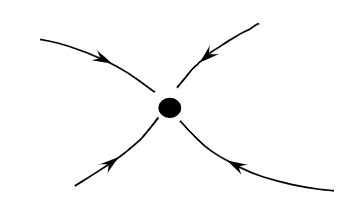
\includegraphics[width=4cm]{FixpunktAttraktor.png}
            & 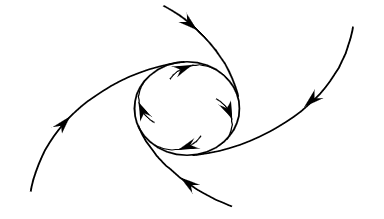
\includegraphics[width=4cm]{GrenzzyklusAttraktor.png}
            & 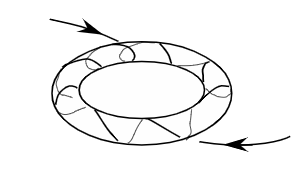
\includegraphics[width=4cm]{TorusAttraktor.png}
        \end{tabular}
        \captionof{figure}{Fixpunkt, Grenzzyklus, Tours- bzw. Ringattraktor \citep{Lueck}}
        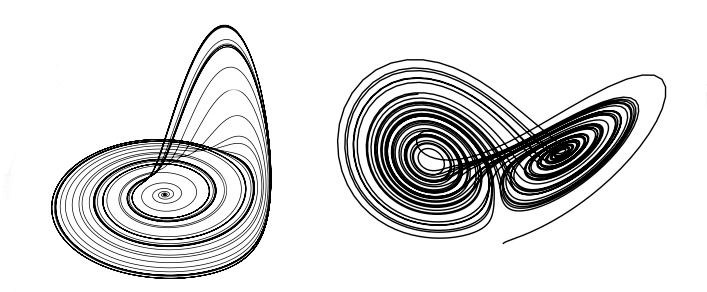
\includegraphics[width=14cm]{SeltsameAttraktoren.png}
        \captionof{figure}{Seltsame Attraktoren: Rössler- und Lorentzattraktor, Eigens erstellt mit dem Python Packages matplotlib mit Hilfe von \citep{py1, py2}}
    \end{center}
\end{itemize}

\subsection{Deterministisches Chaos}
\label{sub:determChaos}
Systeme, die das Verhalten des \textit{deterministischen Chaos} zeigen, weisen ein zufällig erscheinendes Verhalten auf, was jedoch nicht durch äußere Umstände verursacht wird, sondern das Verhalten folgt aus den Eigenschaften des Systems selbst.\\
Das Verhalten von einem System mit deterministischem Chaos lässt sich langfristig nicht vorhersagen, da ähnliche Uhrsachen langfristig nicht zu ähnlichen Wirkungen führen. Das Prinzip der starken Kausalität wird somit verletz \citep{Lueck}.

\subsection{Fouriertransformation und Leistungsspektrum}
\label{sub:fouriertrafo}
Eine Fouriertransformation ist eine Integraltransformation, mit der aperiodische Signale in ein kontinuierliches Spektrum zerlegt werden können.\\
Fouriertransformation einer Messgröße \(x(t)\):
\begin{gather}
    \hat{x}(\omega) = \lim_{T \to \infty} \int_{0}^{T}  x(t) e^{-i\omega t}\,dt 
\end{gather}
Das Leistungsspektrum \( P(\omega)\) kann man nun folgendermaßen aus der Fouriertransformierten des Messwertes berechnen:
\begin{gather}
    P(\omega) = |\hat{x}(\omega)|^2
\end{gather}
Das Leistungsspektrum stellt die Leistungsanteile für unterschiedliche Frequenzen im Zeitsignal dar.\\
Bei chaotischen Systemen beispielsweiße erhält man ein Leistungsspektrum mit kontinuierlichem Verlauf, das für große Frequenzen abnimmt \citep{Lueck}. Da jedoch weißes stochastisches Rauschen ebenfalls ein kontinuierlichen Verlauf liefert kann dieser nicht als hinreichender Beweis für Chaos angesehen werden.

\subsection{Darstellungsweisen eines chaotischen Attraktor}
\label{sub:darstellungAttraktor}
\begin{itemize}
    \item[\textbf{1.}]{\textbf{Phasenraumdarstellung}}\\
    Die \textit{\textbf{Phasenraumdarstellung}} wie in (\ref{sec:allgemeines}) erwähnt, gibt einen Überblick über den Verlauf der Bewegung des dynamischen Systems. Dabei trägt man je an eine Raumachse eine Phasenraumvariabel auf (z.B. $x, \dot{x}$), wobei der Phasenraum dabei $n$-Dimensionen haben kann und nicht alle Phasenraumvariablen bekannt sein müssen, da ein Attraktor im Phasenraum rekonstruiert werden kann. Dazu werden die Messwerte einer Phasenraumvariablen bei einer festen Zeitspanne $\tau$, also $\varphi(t), \varphi(t+\tau)$,..., $\varphi(t+(n-1)\tau)$, als neu Koordinaten $x_i$ (z.B. $x_1=\varphi(t)~\text{und}~x_2=\varphi(t+\tau))$ eines neuen Koordinatensystems. Bei richtiger Wahl von $\tau$ und $n$ lässt sich dann der tatsächliche Attraktor rekonstruieren. Diese Methode der Rekonstruktion eines Atrraktors wurde vom Mathematik \textit{Floris Takens} bewiesen und ist auch als \textit{Einbettungstheorem} bekannt \citep{Lueck}.
    \item[\textbf{2.}]{\textbf{Poincar\'e-Abbildung}}\\
    Die \textit{\textbf{Poincar\'e-Abbildung}} ist eine Projektion des \textit{\textbf{Poincar\'e-Schnitts}} an einer Ebene. Diese Abbildung ist immer die Dimension $n-1$ und ist somit eine Dimension niedriger als der Phasenraum mit der Dimension $n$ und es gehen keinen Informationen bzgl. dem Langzeitverhalten des Systems verloren. Aufgrund dieser Tatsache lässt sich die \textit{Poincar\'e-Abbildung} zur Analyse von höherdimensionalen Phasenräumen verwenden.\\
    Der \textit{Poincar\'e-Schnitt} ist dabei eine Menge aller Durchstoßpunkte der Trajektorien im Phasenraum auf einer Hyperfläche. Hierbei müssen die Trajektorien die Hyperfläche \textit{transversal} (senkrecht) und in einer vorgegebenen Richtung schneiden. Praktisch werden meistens die Lage von Extremwerten einer Messgröße als Bedingung für die Schnittebene (Hyperfläche) und trägt diese gegen die anderen Phasenraumvariablen zu diesem Zeitpunkt gegeneinander auf oder man wählt eine Ebene, die den Attraktor geeignet schneide \citep{Lueck}.
    \item[\textbf{3.}]{\textbf{Wiederkehr-Abbildung}}\\
    Bei der \textit{\textbf{Wiederkehr-Abbildung}} wird eine diskrete Abbildung aktueller Messwerte über die vorangegangenen Messwerte aufgetragen. Dabei werden Punkte in einer $x(n)$-$x(n+1)$-Ebene aufgetragen mit den Messwerten $x_n$ als Koordinaten, also ($x_0,x_1$), ($x_1,x_2$),...,($x_n,x_{n+1}$). Diese Abbildung ähnelt dann einem \textit{Poincar\'e-Schnitt}, weswegen man bei einem kontinuierlichen System (\ref{eq:dynamDGL}) dessen \textit{Poincar\'e-Abbildung} für dieses Verfahren verwendet \citep{Lueck}.
    % TODO: #37 Recherche + Quelle zu Wiederkehrabbildung @ManeLippert
    \item[\textbf{4.}]{\textbf{Bifurkationsdiagramm}}\\
    Bei einem \textit{\textbf{Bifurkationsdiagramm}} betrachtet man die Projektion der \textit{Poincar\'e-Abbildung} auf \textbf{eine} Achse unter Veränderung eines Kontrollparameters, Parameter welche man aktiv im Experiment verändern kann, wobei man die durch die Projektion gewonnenen Werte gegen den jeweiligen Parameterwert aufträgt \citep{Lueck}.
    \newpage
    \item[\textbf{5.}]{\textbf{Phasendiagramm}}\\
    Wenn bei dem \textit{Bifurkationsdiagramm} mehrere unterschiedliche voneinander unabhängige Parameter existieren, verwendet man das \textit{\textbf{Phasendiagramm}}. Dazu trägt man die als Koordinatenachsen die jeweiligen Parameter, die das Systemverhalten beeinflussen, gegeneinander auf und erhält Landkarte des globalen Systemverhaltens in Abhängigkeit der gewählten Parameter \citep{Lueck}.  
\end{itemize}
% Manuel Lippert - Paul Schwanitz
% Physikalisches Praktikum

% Teilaufgabe 2

\section{Das invertierte Pendel}
\label{sec:invertPendel}
Das invertierte Pendel erzeugt eine \textit{nichtlinearer} Schwingung. Dabei besitzt das Pendel eine unten fest eingespannte Blattfeder mit Federkonstante $k$, welche über zwei horizontal in der Höhe $h$ und der Auslenkung $x_h$ angreifende Spiralfedern mit Federkonstante $k_s$ und der Auslenkung $\hat{x}$ angetrieben wird. Am oberen Ende der Blattfeder lässt sich ein Zusatzgewicht $M$ anbringen und der Winkel $\theta$ beschreibt den Winkel zwischen der Tangenten an der Pendelspitze und dem Lot. Weiterhin bezeichnet die Pendellänge $L$ die Länge zwischen dem Anfang und Ende der Blattfeder, welche vom Winkel $\theta$ abhängt (siehe Abb \ref{image:invertiertesPendel}).
\begin{center}
    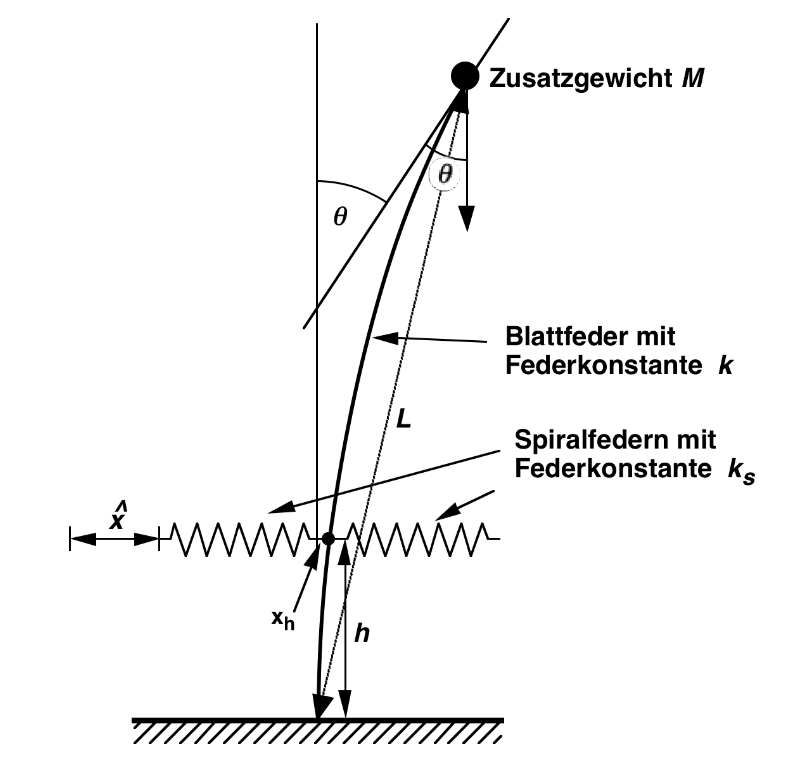
\includegraphics[scale=0.25]{Pendel/invertiertesPendel.png}
    \captionof{figure}{Skizze invertiertes Pendel \citep{Lueck}}
    \label{image:invertiertesPendel}
\end{center}
\subsection{Herleitung der Bewegungsgleichung}
\label{sub:bewegungsgleichung}
Die Bewegungsgleichung lässt sich über die wirkenden Drehmomente der Bauteile bestimmen:
\begin{gather*}
        \text{Pendel}~+~\text{Dämpfung}~+~\text{Blattfeder}~-~\text{Spiralfedern}~-~\text{Gewicht} = 0
\end{gather*}
\begin{gather}
    \Rightarrow [M(L(\theta))^2\ddot{\theta}]+[2\delta\dot{\theta}]+[k\theta]-[hk_s(x_h+\hat{x}\cos(\omega t))]-[MgL(\theta)\sin(\theta)]=0
\end{gather}
Dabei bezeichnet $\delta$ die Dämpfungskonstante und $g$ die Erdbeschleunigung.\\
Im Folgenden wird die Pendellänge $L$ als konstant angenommen, obwohl diese nicht konstant ist und von der Art der verwendeten Masse $M$ abhängt. Weiterhin wird die Auslenkung $x_h$ als vernachlässigbar klein angesehen und der Angriffswinkel der Spiralfedern wird als $\frac{\pi}{2}$ genähert, was bei genügend kleiner Höhe $h$ gegeben ist.
Daraus folgt die genäherte Form der Bewegungsgleichung:
\begin{gather}
    ML^2\ddot{\theta}+2\delta\dot{\theta}+k\theta-MgL(\theta)\sin(\theta)=hk_s\hat{x}\cos(\omega t)=T_0\cos(\omega t)
\end{gather}
Wobei $T_0$ als die Amplitude des periodisch angreifenden Drehmoments interpretiert werden muss. Hierbei ist noch zu erwähnen, dass durch die Näherungen die Lösung dieser Differentialgleichung nicht der tatsächlichen Trajektorien des Systems entsprechen, da diese stark von der Anfangsbedingung abhängen, dennoch ist eine globale Aussage über das Verhalten mit der genähreten Differentialgleichung möglich.\\
Zu den letzten beiden Termen lässt sich dann ein Potenzial definieren und durch Entwicklung des Cosinus für kleine Winkel $\theta$ (Kleinwinkelnäherung KWN) bis zur 2.Ordnung ergibt sich das Potenzial des \textit{Duffing-Oszillator} \citep{Lueck}.
\begin{gather}
    V(\theta) = \frac{1}{2}k\theta^2 + MgL(\cos(\theta)-1)\overset{\text{KWN}}{\approx}\frac{1}{2}(k-MgL)\theta^2 + \frac{1}{24}MgL\theta^4~,V(0)=0
\end{gather}

\subsection{Symmetriebrechung}
\label{sub:symbrechung}
Bei einer {kritischen Masse} $M_k=\frac{k}{gL}$ erfährt das System des Pendels einen Übergang von einem monostabilen System ($M<M_k$) in ein bistabiles System ($M>M_k$), dabei ist die Bewegung des Pendels in beiden Fällen Unterschiedlich und muss deshalb getrennt betrachtet werden. Bei diesem Übergang verändert sich die Struktur des Potenzial (siehe Abb \ref{image:potPendel}), wodurch nun zwei Lösungen für das System möglich sind. Das Auftreten von mehreren Lösungen in einem System wird dann auch \textit{\textbf{Symmetriebrechung}} genannt \citep{Lueck}.
\begin{center}
    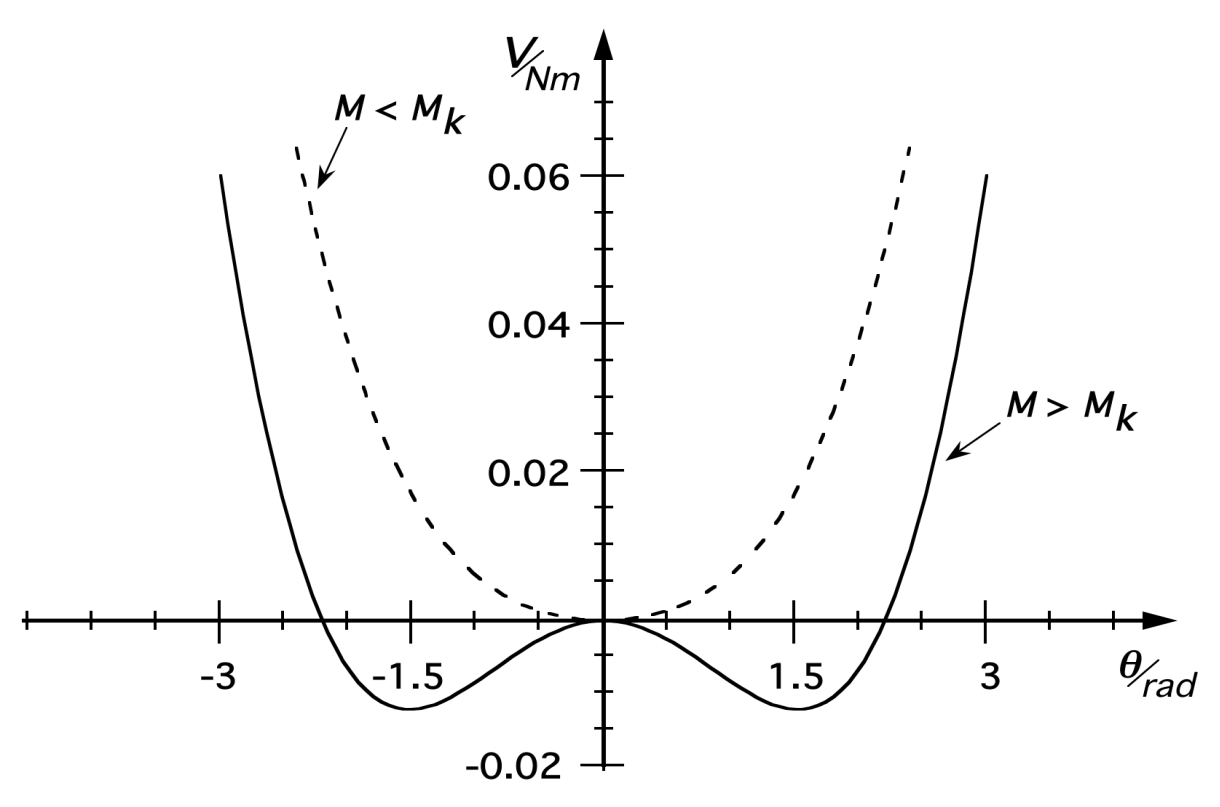
\includegraphics[scale = 0.2]{Pendel/PendelPotenzial.png}
    \captionof{figure}{Potenzialdarstellung für invertiertes Pendel \citep{Lueck}}
    \label{image:potPendel}
\end{center}

\subsection{Schwingungsdauer in Abhängigkeit der Masse}
\label{sub:schwingungsdauer}
Bei einem nichtlinearen Pendel hängt, im Gegensatz zu einem linearen Schwingungsvorgang, die Resonanzfrequenz $\omega_r$ von der Schwingungsamplitude $b$ ab $\Rightarrow \omega_r(b)$. Unverändert bleibt dennoch die Schwingungsamplitude $b(\omega)$ gegenüber der Resonanzkurve eines linearen Oszillators bei unterschiedlichen Anregungsfrequenzen $\omega$ \citep{Lueck}.
\begin{itemize}
    \item[1.] $M<M_k$ (Schwache Nichtlinearität)\\
    Pendel ist nach (\ref{sub:symbrechung}) monostabil. Der Vorgang lässt sich näherungsweise mit der Bewegungsgleichung eines Duffing-Oszillator nähern, wobei die Abhängigkeit der Resonanzfrequenz $\omega_r$ von der Amplitude $b$ berücksichtigt bleibt. Die Bewegungsgleichung lautet in diesem Fall:
    \begin{gather}
        \ddot{\theta} + 2\delta\dot{\theta} + \omega_0^2\theta + \gamma\theta^3 = f_a\cos(\omega t)
    \end{gather}
    Dabei bezeichnet $\gamma$ den Faktor der Nichtlinearität, $\omega_0$ die Resonanzfrequenz des Systems ohne Nichtlinearität ($\gamma=0$), $f_a$ die Anregungsamplitude mit Anregungsfrequenz $\omega$ und $\delta$ die Dämpfung.\\
    Durch Betrachtung des Verlaufs der Resonanzkurve in der Nähe von $\omega_0$ erhält man eine Gleichung dritter Ordnung für das Quadrat der Schwingungsamplitude $b$.
    \begin{gather}
        \left[\left((\omega^2-\omega_0^2) - \frac{3}{4}\gamma b^2\right)^2+(2\delta\omega)^2\right]b^2=f_a^2 %Angepasst an die Form in Wikipedia https://en.wikipedia.org/w/index.php?title=Duffing_equation&oldid=1031816809
        \label{eq:resonanzkurve}
    \end{gather}
    Diese Gleichung hat je nach Werten von $f_a, \gamma, \omega_0~\text{und}~\delta$ eine reelle oder zwei konjugierte komplexe Lösungen.
    Dabei ist es einfacher die Gleichung nach $\omega$ aufzulösen, wobei zur Vereinfachung $\omega_0=1$ angenommen wird. Damit wird (\ref{eq:resonanzkurve}) zu:
    \begin{gather}
        \left[\left((\omega^2-1) - \frac{3}{4}\gamma b^2\right)^2+(2\delta\omega)^2\right]b^2=f_a^2
    \end{gather}
    Mit der Lösung für $\omega$:
    \begin{gather}
        \omega^2_{1,2} = 1 - 2\delta^2 + \frac{3}{4}\gamma b^2 \pm \sqrt{\frac{f_a^2}{b^2}+ 4\delta^2\left[\delta^2 - \left(1 + \frac{3}{4}\gamma b^2\right)\right]}
    \end{gather}
    Bei hinreichender kleinen Dämpfung $\delta$ gibt es zwei verschiedene eingeschwungene Zustände, da die Lösung instabil wird (siehe Abb \ref{image:resonanzkurve}c)).
    \begin{center}
        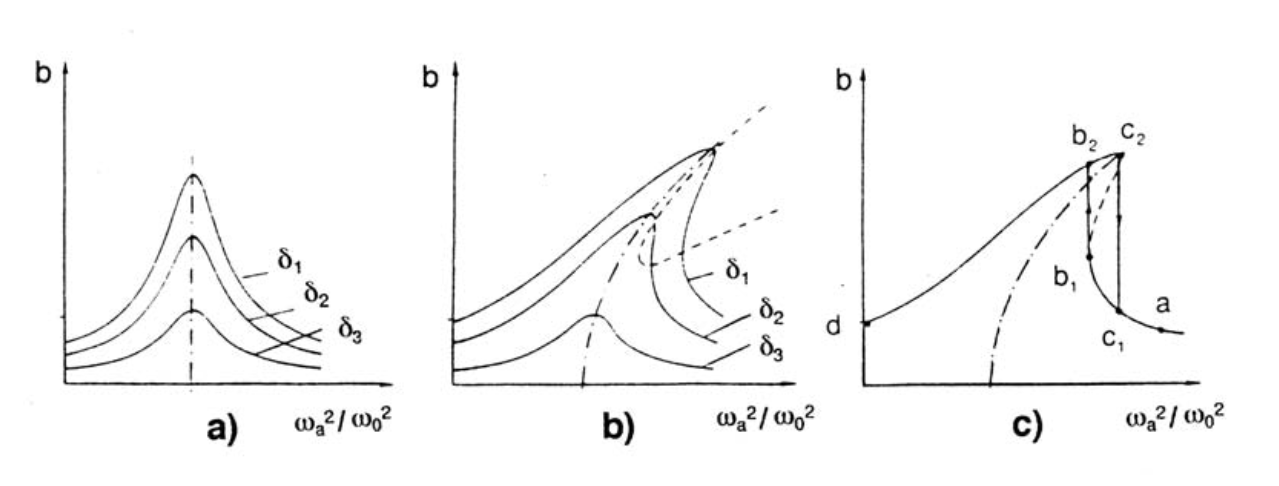
\includegraphics[scale=0.3]{Pendel/Resonanzkurve.png}
        \captionof{figure}{Resonanzkurven für eines Duffing-Oszillator \citep{Lueck}}
        \label{image:resonanzkurve}
        \captionof*{figure}{a) linearer ($\gamma=0$) b) nichtlinear c) Hysterese}
    \end{center}
    % https://www.ila.uni-stuttgart.de/nlvib/downloads/HB_NLvib_presentation.pdf, https://www.hindawi.com/journals/mpe/2011/248328/
    Die Schwingungsdauer $T$ hängt hierbei logarithmisch von der Amplitude $b$ ab mit dem Zusammenhang:
    \begin{gather}
        T = T_0 + T_1\log(b)
    \end{gather}
    Dies geht aus experimentellen Daten von \citep{Lueck} hervor, wobei $T_0$ und $T_1$ Näherungsparameter sind.
    \item[2.] $M>M_k$ (Starke Nichtlinearität)\\
    Das Pendel ist in diesem Fall nach (\ref{sub:symbrechung}) bistabil und besitzt zwei stabile Ruhelagen. Durch die Verringerung von großen Antriebsfrequenzen $\omega$ entstehen nach Ende des Einschwingverhaltens nacheinander subharmonische Schwingungen mit einer Periodenverdopplungskaskade ($T_n=2^nT=2^n\frac{2\pi}{\omega}$), obwohl sich das Pendel unterhalb einer kritischen Frequenz $\omega_k$ chaotisch verhält. Dieses Verhalten ist auch ein Beispiel für ein Bifurkationsszenario \citep{Lueck}.
\end{itemize}
\newpage
\subsection{Aufbau Pendel}
\label{sub:aufbauPendel}
\begin{center}
    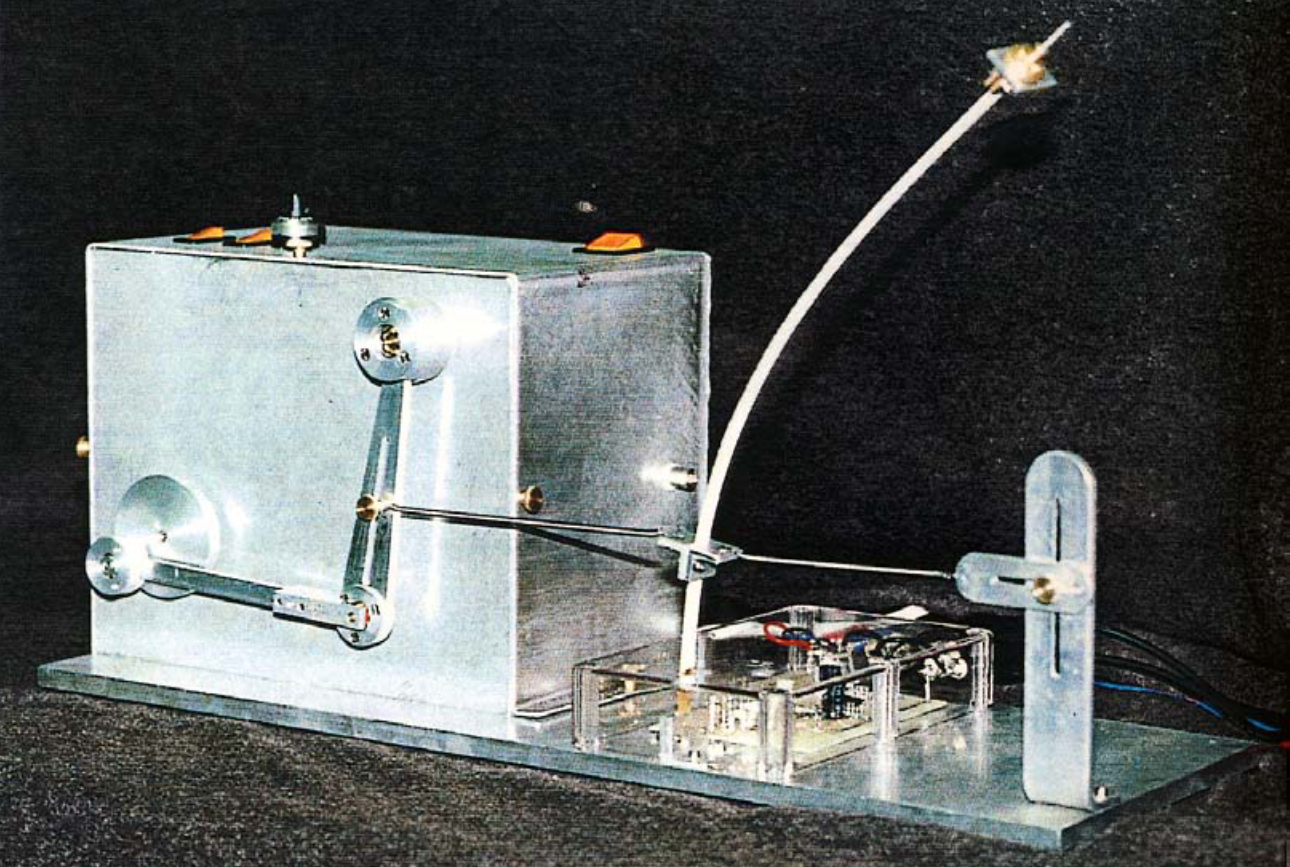
\includegraphics[scale=0.25]{Pendel/AufbauPendel.png}
    \captionof{figure}{Aufbau des invertierten Pendels \citep{Lueck}}
    \label{image:aufbauPendel}
\end{center}
Hierbei besteht das Pendel aus einer:
\begin{itemize}
    \item 5 mm starken Aluminium-Grundplatte
    \item 1 cm x 15 cm x 40 cm lange Blechstreifen aus einer Messing-Legierung mit hohem Kupferanteil, Dehnungsmessstreifen auf beiden Seiten (DMS, Widerstand abh. von der Dehnung) knapp oberhalb der Befestigung $\rightarrow$ Blattfeder
    \item Spiralfedern mit Federkonstante $k=027$ N/cm 
    \item Schrittmotor im Gehäuse mit 200 bzw. 400 Schritten (Halbschrittbereich)
    \item Multifunktionskarte Typs DAS 1602 der Firma Keithley (Taktimpulsgeber für Schrittmotoren)
\end{itemize}
Mit diesem Aufbau sind bis zu ca 5 Umdrehungen/s möglich, wobei die Antriebskraft durch das Verändern des Angriffspunktes der Spiralfeder am Übertragungshebel variierbar ist \citep{Lueck}.

\subsection*{Funktionsweise Differenzier-Schaltung}
Bei einer Differenzier-Schaltung wird nur die Änderung der Eingangsspannung zu einer Ausgangsspannung verarbeitet. Dabei wird ein Kondensator am Eingang in Reihe und ein Widerstand parallel zwischen Eingang und Ausgang des Operationsverstärker geschaltet. Durch den Kondensator fließt nur Strom, wenn sich die Eingangsspannung ändert, wobei die Ausgangsspannung proportional zur Änderungsgeschwindigkeit der Eingangsspannung ist. Durch den Operationsverstärker wird dann das Signal verstärkt, um dieses Signal besser über ein angeschlossenes Messgerät (z.B. Oszilloskop) betrachten zu können \citep{electronik}.

\begin{center}
    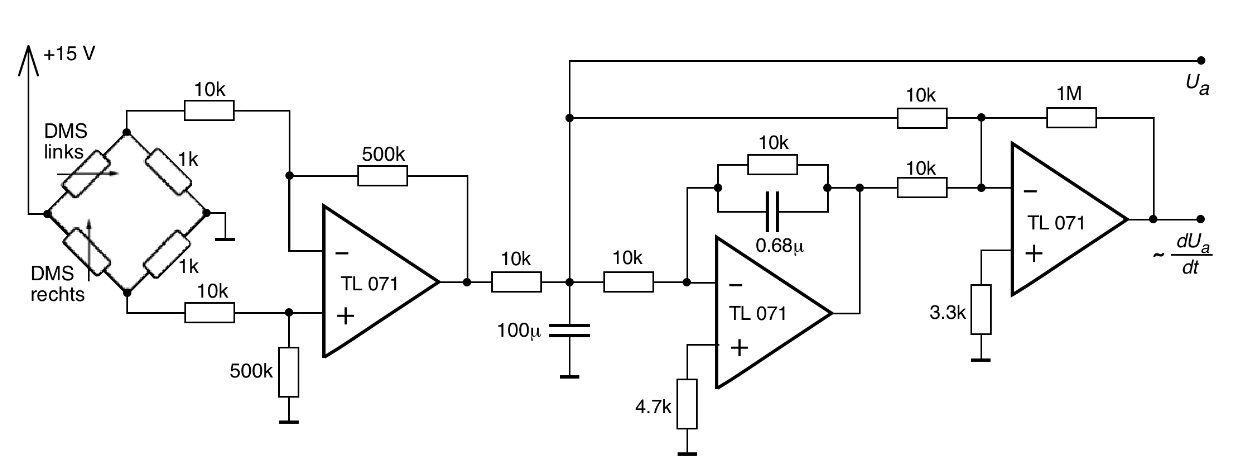
\includegraphics[scale=0.3]{Pendel/MessschaltungPendel.png}
    \captionof{figure}{Messschaltung des invertierten Pendels \citep{Lueck}}
    \label{image:schaltungPendel}
\end{center}
Für die Messschaltung (siehe Abb. \ref{image:schaltungPendel}) wird für eine höhere Genauigkeit zwei DMS in einer Brückenschaltung verschalten, um die Spannungsdifferenz von ihnen zu messen, wobei die Spannung dann proportional zur Pendelauslenkung $\theta$ ist. Für das Abgreifen der Geschwindigkeit als zweite Phasenraumvariable werden die Spannungen über eine Operationsverstärker-Schaltung differenziert. Die Spannungen werden dann einem im PC eingebauten Analog-Digital-Wandler-Karte gemessen, wobei die Messkarte über LABVIEW (Messprogramm) gesteuert wird \citep{Lueck}.
% Manuel Lippert - Paul Schwanitz
% Physikalisches Praktikum

% Teilaufgabe 3
\newpage
\section{Der Shinriki-Oszillator}
\label{sec:shinrikiOszi}


\subsection{Differentialgleichung und Aufbau des Shinriki-Oszillator}
\label{sub:dgl}

\begin{figure}[h]
    \centering
    %TODO #31
    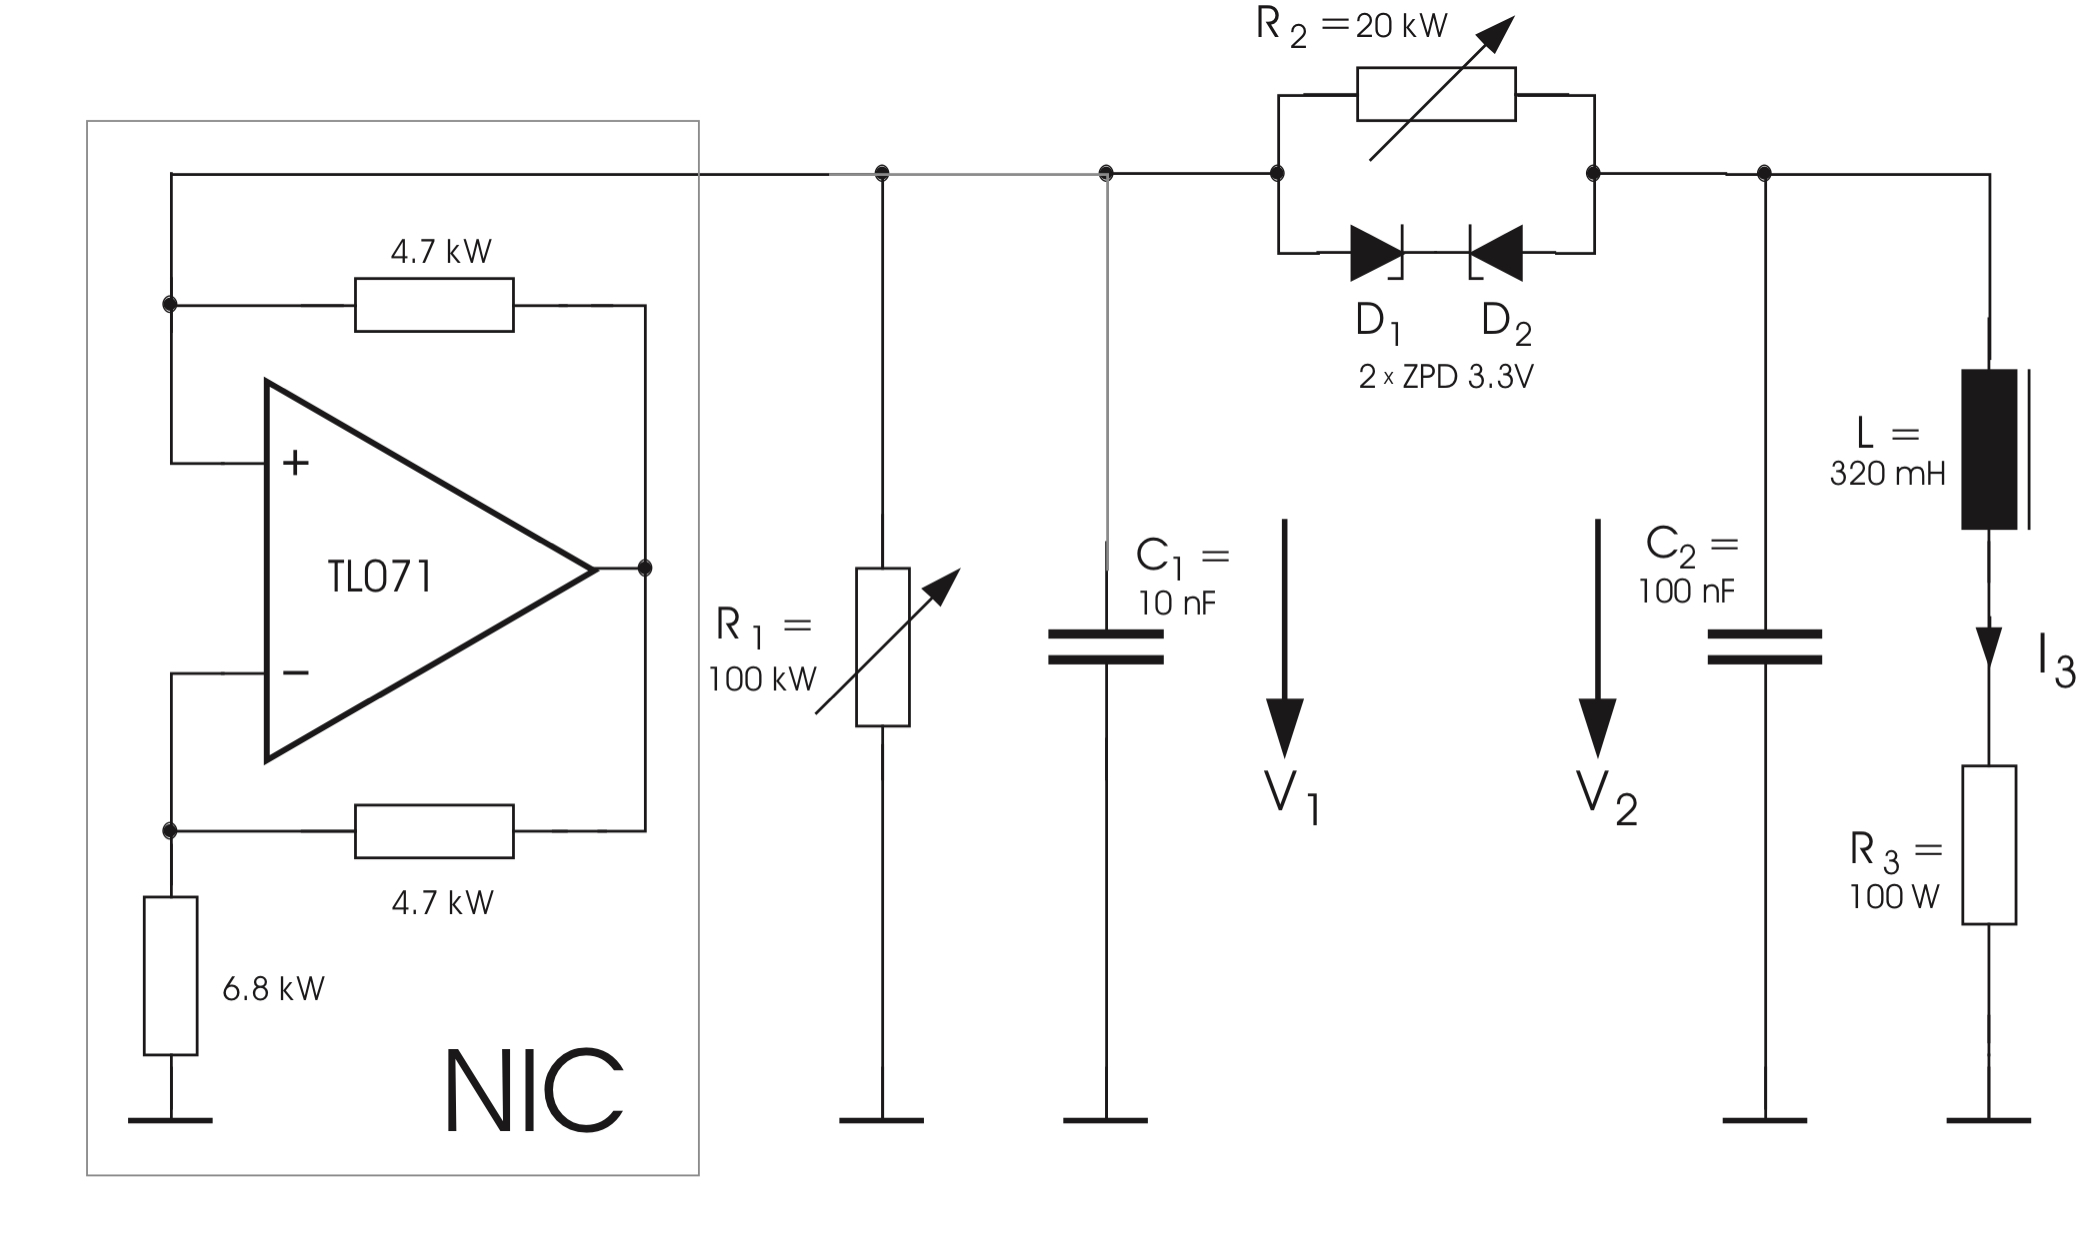
\includegraphics[scale=0.15]{ShinrOsziSp.jpeg}
    \label{fig:shinrikiSp}
    \caption{Schaltplan des Shinriki-Oszilator \citep{Lueck}}
\end{figure}

Der Shinriki-Oszillator besteht aus einem negativen Impedanzkonverter (NIC) und einem LC-Parallelschwinkreis, die durch ein gegeneinader geschaltetes Zenerdiodenpaar und dem parallel geschalteten \(R_2\), gekoppelt sind. \\
Die Leitwertfunktion des Kopplungsglied ist \( f(V)\) und beschreibt den Strom, der über das Kopplungsglied fließt.
\(R_{NIC}\) ist der Widerstand des NIC innerhalb des relevanten Intervalls von -8,1 V bis 8,1 V \citep[]{Lueck}.\\
Damit und mit den Kirchhoffschen Regeln lassen sich nun die DGLs aufstellen:
\begin{align}
    C_1 \dot{V_1} &= V_1 (\frac{1}{R_{NIC}}-\frac{1}{R_1}) - f(V_1-V_2) \\
    C_2 \dot{V_2} &= f(V_1-V_2) - I_3 \\
    L \dot{I_3} &= -I_3R_3 + V_2
\end{align}

\subsection{NIC und Schwingung des Shinriki-Schaltkreis}
\label{sub:nic}
Ein NIC benutzt einen Operationsverstärker, um einen negativen ohmschen Wiederstand zu simulieren. Hierbei wird der gewünschte Widerstand einfach zwischen dem (-) Eingang des OpAmp und GND geschaltet. Durch den OpAmp wird ein Widerstand mit negativem Wert des eben eingesetzten simuliert. \\
Daher mus das System nicht mehr von außen zur Schwingung angeregt werden.
% TODO #29

\subsection{Geräusche einer Bifurkation}
\label{sub:tonBifurkation}
Eine Bifurkation ist eine verdopplung der Periodendauer, d.h. die Frequenz wird halbiert. Dies verursacht einen tieferen Ton.
% TODO #30

% etc.

    % 3.Kapitel Protokoll
    % Charlotte Geiger - Manuel Lippert - Leonard Schatt
% Physikalisches Praktikum

% 3.Kapitel  Protokoll

% Variables
\def\skalierung{0.65}

\chapter{Methodik}
\label{chap:protokoll}
\section{Aufbau}

Der hier verwendete Aufbau besteht aus einem AFM der Marke Nanosurf, einer dazugehörenden Steuerelektronik und einem Computer mit dem 
Programm  'AFM  Nanosurf  Easy  Scan  2'. An diesem kann der Messbereich, der Setpoint, die Zeit pro Zeile und die Anzahl der Zeilen und 
Punkte pro Zeile festgelegt werden. Bilder zum Versuchsaufbau befinden sich im Anhang \ref{section:AnhangAufbau}. \\

\section{Versuchsdurchführung}

Eine Durchführung läuft folgendermaßen ab:\\
Die Probe wird aus ihrer Schachtel genommen und auf die magnetische Platte gegeben. Dann wird mit Hilfe von Millimeterschrauben die Probe unter den Cantilever gefahren. 
Dort wird der Cantilever manuell abgesenkt bis man den Schatten des Cantilevers auf dem Präparat in der Kamera sieht. Danach lässt man den Computer den Cantilever 
automatisch auf die richtige Distanz fahren. Dies geschieht durch eine PI(D)-Regler Schaltung, welche schon voreingestellt war. \\
Anschließend drückt man, nachdem man die entsprechenden Größen eingegeben hat, 'Start' und die Messung läuft von alleine ab. Die Einstellung zur jeweiligen Messung sind unten 
vermerkt.\\
Danach speichert man die Messung als nid-File. Den Angleich der X-Y-Ebene muss man hier nicht manuell durchführen. Diesen übernimmt das Programm automatisch.


\subsection*{Eichgitter}
\begin{center}
    \centering
    \begin{tabular}{l|r}
        Modus & Contact Mode \\
        Image size & 62,65 $\mu$m \\
        Time / Line & 2s \\
        Points/Line & 512\\
        Setpoint & 15 nN \\
        P-Gain & 10000 \\
        I-Gain & 1000 \\
        D-Gain & 0 \\
        
    \end{tabular}
\end{center}

\subsection*{CD-Presswerkzeug}
\subsubsection*{50$\mu$m}
\begin{center}
    \centering
    \begin{tabular}{l|r}
        Modus & Contact Mode\\
        Image size & 50,00 $\mu$m \\
        Time / Line & 2s \\
        Points/Line & 512\\
        Setpoint & 15 nN \\
        P-Gain & 10000 \\
        I-Gain & 1000 \\
        D-Gain & 0 \\
        
    \end{tabular}
\end{center}

\subsubsection*{20$\mu$m}

\begin{center}
    \centering
    \begin{tabular}{l|r}
        Modus & Contact Mode\\
        Image size & 19,34 $\mu$m \\
        Time / Line & 2s \\
        Points/Line & 512\\
        Setpoint & 15 nN \\
        P-Gain & 10000 \\
        I-Gain & 1000 \\
        D-Gain & 0 \\
        
    \end{tabular}
\end{center}

\subsection*{Nanotubes}
\subsubsection*{15$\mu$m}

\begin{center}
    \centering
    \begin{tabular}{l|r}
        Modus & Contact Mode\\
        Image size & 15,00 $\mu$m \\
        Time / Line & 1,3s \\
        Points/Line & 512\\
        Setpoint & 3,02 nN \\
        P-Gain & 10000 \\
        I-Gain & 1000 \\
        D-Gain & 0 \\
        
    \end{tabular}
\end{center}

\subsubsection*{2$\mu$m}

\begin{center}
    \centering
    \begin{tabular}{l|r}
        Modus & Contact Mode\\
        Image size & 2,168 $\mu$m \\
        Time / Line & 1,3s \\
        Points/Line & 512\\
        Setpoint & 3,02 nN \\
        P-Gain & 10000 \\
        I-Gain & 1000 \\
        D-Gain & 0 \\
        
    \end{tabular}
\end{center}

\subsection*{Goldcluster}

\subsubsection*{2,5 $\mu$m}
\begin{center}
    \centering
    \begin{tabular}{l|r}
        Modus & Non-Contact Mode\\
        Image size & 2,5 $\mu$m \\
        Time / Line & 1s \\
        Points/Line & 512\\
        Setpoint & 60\% \\
        P-Gain & 10000 \\
        I-Gain & 1000 \\
        D-Gain & 0 \\
        
    \end{tabular}
\end{center}

\subsubsection*{1,5 $\mu$m}
\begin{center}
    \centering
    \begin{tabular}{l|r}
        Modus & Non-Contact Mode\\
        Image size & 1,5 $\mu$m \\
        Time / Line & 1s \\
        Points/Line & 512\\
        Setpoint & 70\% \\
        P-Gain & 10000 \\
        I-Gain & 1000 \\
        D-Gain & 0 \\
        
    \end{tabular}
\end{center}

\subsubsection*{0,375 $\mu$m}
\begin{center}
    \centering
    \begin{tabular}{l|r}
        Modus & Non-Contact Mode\\
        Image size & 0,375 $\mu$m \\
        Time / Line & 1s \\
        Points/Line & 512\\
        Setpoint & 70\% \\
        P-Gain & 10000 \\
        I-Gain & 1000 \\
        D-Gain & 0 \\
        
    \end{tabular}
\end{center}

\subsection*{Oberflächengitter}

\begin{center}
    \centering
    \begin{tabular}{l|r}
        Modus & Non-Contact Mode\\
        Image size & 20 $\mu$m \\
        Time / Line & 1,75s \\
        Points/Line & 512\\
        Setpoint & 60\% \\
        P-Gain & 10000 \\
        I-Gain & 1000 \\
        D-Gain & 0 \\
        
    \end{tabular}
\end{center}

\subsection*{PSPMMA}

\begin{center}
    \centering
    \begin{tabular}{l|r}
        Modus & Non-Contact Mode, Phase Contrast\\
        Image size & 2 $\mu$m \\
        Time / Line & 1s \\
        Points/Line & 512\\
        Setpoint & 70\% \\
        P-Gain & 10000 \\
        I-Gain & 1000 \\
        D-Gain & 0 \\
        
    \end{tabular}
\end{center}




\section{Geräte und Fehler}

Rasterkraftmikroskop: Inventarnummer: 88459\\
Steuerelektronik: Inventarnummer: 88080\\
Cantilever (Contact Mode): NANOSENSORS type PPP-CONT nachdeR-C, S/N 78932F10L995, vom 31.7.14, Set 5\\
Cantilever (Non-Contact): NANOSENSORS, Type PPP-NCLR-10, S/N 66017F4L734
Eichgitter: Nummer: BT00250, x-y-Periodizität: 10,0 $\mu$m, z-Höhe: 119nm, Batch: 2003-03-29.2
Diverse Proben: Nanosurf Extended Sample Kapitel\\
Oberflächengitter: Gitter(1.9.14)



% Einbindung des Protokolls als pdf (mit Seitenzahl etc.)
% Erste Seite mit Überschrift
%\includepdf[pages = 1, landscape = false, nup = 1x1, scale = \skalierung , pagecommand={\thispagestyle{empty}\chapter{Protokoll}}]
%            {03-Protokoll/Protokoll.pdf}
% Restliche Seiten richtig skaliert
%\includepdf[pages = -, landscape = false, nup = 1x1, scale = \skalierung , pagecommand={}]
%            {03-Protokoll/Protokoll.pdf}

    % 4.Kapitel Versuchsauswertung
    % Matteo Kumar - Leonard Schatt
% Fortgeschrittenes Physikalisches Praktikum
% 4.Kapitel Versuchsauswertung

\chapter{Auswertung und Diskussion}
\label{chap:versuchsauswertung}

% Text

% Input der Teilauswertung je nach Produktion der Nebendateien ohne Ordner
%Matteo Kumar - Leonhard Schatt
% Fortgeschrittenes Physikalisches Praktikum

% Teilauswertung Eichgitter

\section{Vermessung eines Eichgitters}
\subsection{x-y-Verschiebung}
Zuerst soll das Eichgitter vermessen und die Messergebnisse mit den Herstellerangaben verglichen werden. Dazu wird die Aufnahme des AFM mit 
Gwyddion \footnotemark \footnotetext{\url{http://gwyddion.net/}} geöffnet und untersucht.\\
Zur Bestimmung der x-y-Verschiebung werden Strecken über mehrere Raster hinweg und einzelne Raster wie in Abb. \ref{bild:EichWo} gezeigt 
gemessen. 

\begin{figure}[h]
    \centering
    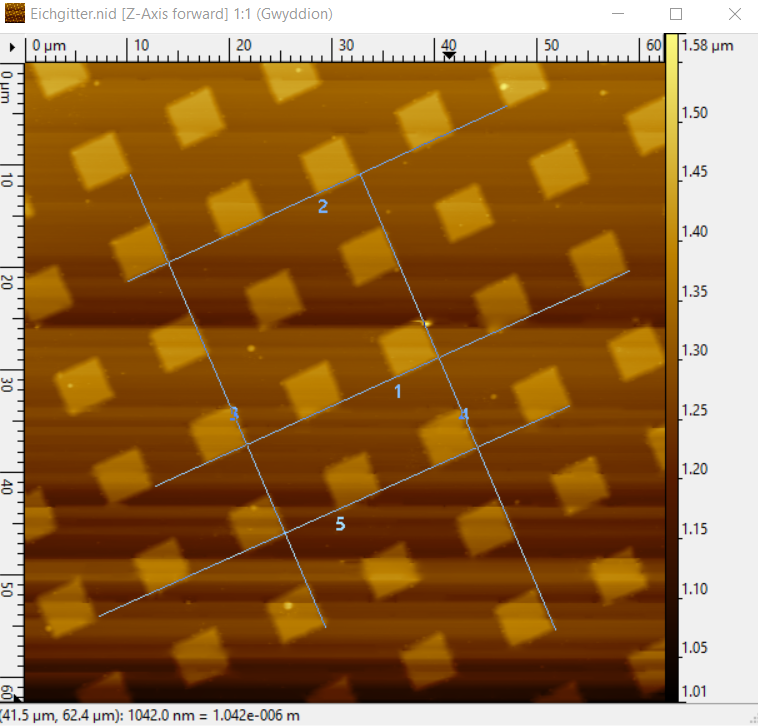
\includegraphics[scale = 0.5]{Bilder/EichGeraden.png}
    \caption{Lage der vermessenen Geraden im Eichgitter}
    \label{bild:EichWo}
\end{figure}
\newpage

Die Längen der Strecken sind:

\begin{center}
    \centering
    \begin{tabular}{l|r r}
        Nummer & Strecke / $\mu m$ & Anzahl Raster \\
        \hline
        1 & 50.9 & 10\\
        2 & 40.8 & 8\\
        3 & 48.2 & 10 \\
        4 & 48.4 & 10 \\
        5 & 50.3 & 10\\
        
    \end{tabular}
\end{center}

Aus den Längen lässt sich der Mittelwert für eine x-y-Versetzung berechnen.

\begin{equation*}
    d_{xy} = 9.942 \mu m
\end{equation*}

Der Hauptfehler dürfte beim Wählen der Start- und Endpunkte 
der zu vermessenden Strecke liegen, da diese nicht sehr gut exakt zu setzen waren. Mithilfe des Vermessungstools wird dieser Fehler auf 
2$\mu m$ pro Strecke abgeschätzt. Nach Fehlerfortpflanzung ergibt sich also:
\begin{equation*}
    s = \sqrt{5}\frac{2 \mu m}{24} = 0.186 \mu m
\end{equation*}

Mit dem internen Fehler des Mikroskops von 1.2\%, ergibt sich für die Versetzung ein Fehler von
\begin{equation*}
    s_d = \sqrt{0.186^2 + (0.012 \cdot 9.942)^2}\, \mu m = 0.22\, \mu m
\end{equation*}

\begin{equation*}
    \textcolor{red}{d_{xy} = (9.94 \pm 0.22) \mu m}
\end{equation*}

Nach Angaben des Herstellers beträgt die Versetzung 10.0 $\mu m$ (s. Protokoll). 
Dieser Wert liegt innerhalb des Fehlers, deshalb kann er als bestätigt angesehen werden. Auffällig ist allerdings, dass sich, 
wenn man die Versetzungen für 'horizontale' (1,2,5) und 'vertikale' (3,4) Strecken getrennt berechnet, unterschiedliche Werte ergeben: 
\begin{equation*}
    d_{xy,h} = 10.14 \mu m, \qquad d_{xy,v} = 9.66 \mu m
\end{equation*}

Dies kann nicht nur Folge von Ungenauigkeiten beim Wählen von den Endpunkten der Strecke sein, dafür ist der berechnete Fehler zu gering. 
Möglich wäre auch noch eine Verkippung des Gitters, sodass die ausgemessenen x-y-Koordinaten nicht exakt der Strecke auf dem Gitter 
entsprechen. In der Tat ist im Profil des Bildes des Eichgitters ein linearer Trend zu erkennen (Abb. \ref{bild:EichKippung}). 
Da die Ergebnisse dennoch gut mit der Theorie übereinstimmen wird an dieser Stelle auf eine Bereinigung verzichtet.

\begin{figure}[h]
    \centering
    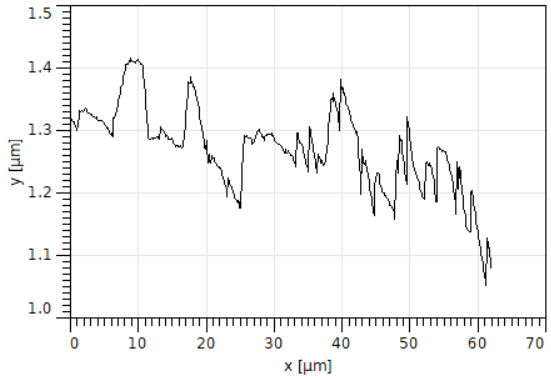
\includegraphics[scale = 0.65]{Bilder/EichKippung.png}
    \caption{Profil des Eichgitters. Ein linearer Trend ist gut zu erkennen - das Gitter ist leicht verkippt.}
    \label{bild:EichKippung}
\end{figure}

\newpage
\subsection{Höhe des Gitters}

Zur Bestimmung der Höhe der Raster wurde ein Höhenprofil von zwei Strecken (s. Abb. \ref{bild:zUebersicht}) erstellt und die Erhöhungen 
vermessen. Die Höhenprofile finden sich in den Abb. \ref{bild:zReihe1} und \ref{bild:zReihe2}. 

\begin{figure}[h]
    \centering
    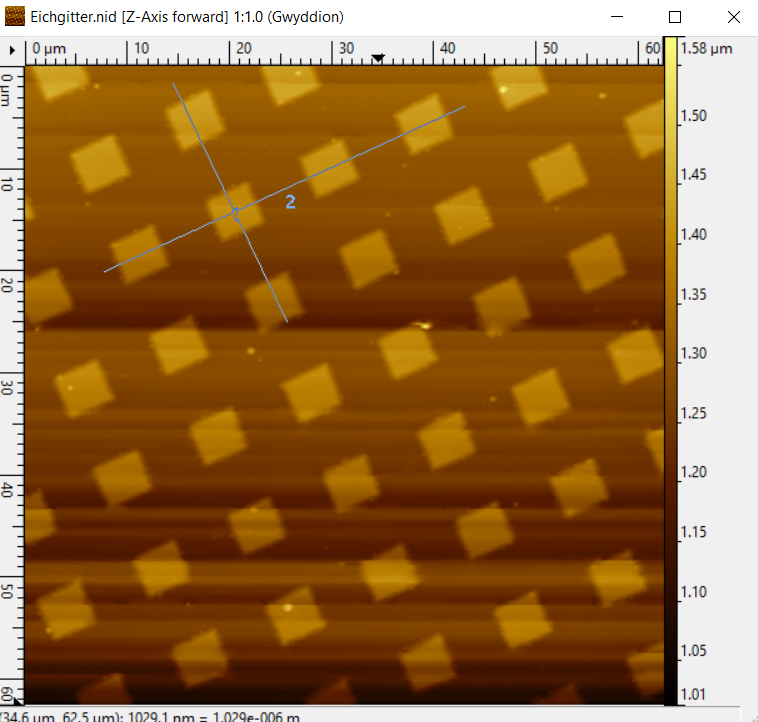
\includegraphics[scale = 0.4]{Bilder/zUebersicht.png}
    \caption{Lage der Geraden zu den Höhenprofilen im Eichgitter}
    \label{bild:zUebersicht}
\end{figure}

\begin{figure}[h]
    \centering
    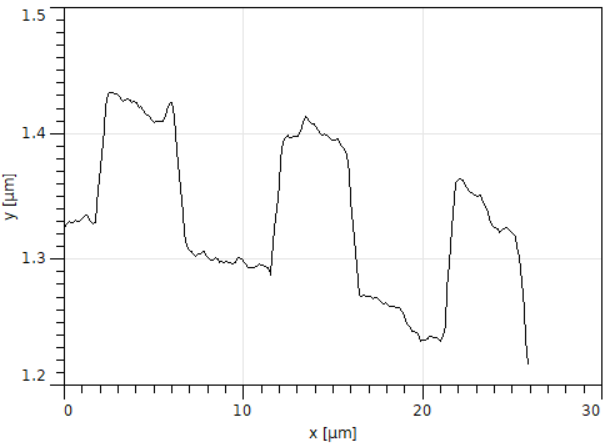
\includegraphics[scale = 0.65]{Bilder/zReihe1.png}
    \caption{Höhenprofil der ersten Geraden}
    \label{bild:zReihe1}
\end{figure}

\begin{figure}[h]
    \centering
    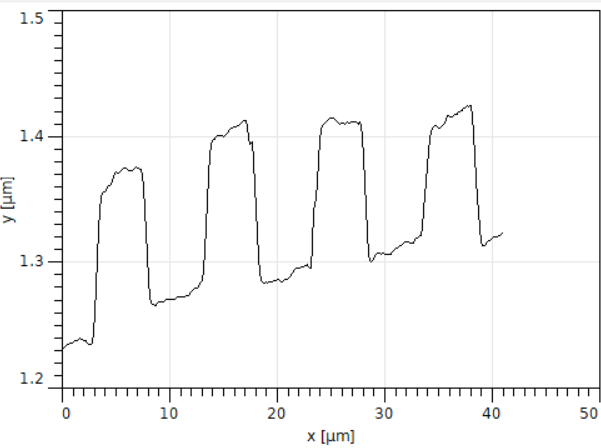
\includegraphics[scale = 0.65]{Bilder/zReihe2.png}
    \caption{Höhenprofil der zweiten Geraden}
    \label{bild:zReihe2}
\end{figure}

\clearpage

Die Höhe der Erhebungen sind: 

\begin{center}
    \centering
    \begin{tabular}{l|r}
        Strecke Reihe 1 /  nm & Strecke Reihe 2 / nm \\
        \hline
        118.0 & 109.6 \\
        107.1 & 119.4 \\
        117.6 & 115.2 \\
        122.3 & 123.7 \\
        119.2 & 128.3 \\
        110.6 & \\
        91.0 & \\
        110.7 & \\
        
    \end{tabular}
\end{center}

Der Mittelwert daraus beträgt $h = 114.823 nm$.
Der Fehler wird hauptsächlich durch die Präzession beim Auswählen der Punkte für die Höhenmessung bestimmt; es war nicht immer klar, 
wo der Anstieg beginnt und endet. Es sei deshalb pro Messung ein Fehler von 5nm angenommen. Über Fehlerfortpflanzung ergibt sich für 
den Fehler des Mittelwerts: 
\begin{equation*}
    s_h = \frac{5}{\sqrt{13}} nm = 1.39 nm
\end{equation*}

Damit ist die Höhe der Erhebungen: 
\begin{equation*}
    \textcolor{red}{h = (114.8 \pm 1.4)nm}
\end{equation*}

Laut Hersteller sollte die Höhe aber 119.0 nm betragen, was außerhalb des Fehlerbereichs liegt (s. Protokoll). Eine Erklärung wäre, dass der Fehler 
zu niedrig abgeschätzt wurde. Wahrscheinlicher ist es aber, dass die Erhöhungen im Laufe der Zeit durch das Vermessen im Contact-Mode 
abgeschliffen wurden. Dafür sprechen auch die an den Helligkeitsunterschieden vor allem in der unteren Hälfte von 
Abb. \ref{bild:zUebersicht} erkennbaren horizontalen Linien über den gesamten Gitterausschnitt. Dies könnten Messfehler des 
AFM sein. Deshalb war auch die Wahl der Strecken für diese Messung nicht ganz einfach, da 
eine Stelle mit möglichst wenig Abnutzung gefunden werden musste. Zum Vergleich ist in Abb. \ref{bild:zUngeeignet} ein dafür 
ungeeignetes Profil zu sehen.

\begin{figure}[h]
    \centering
    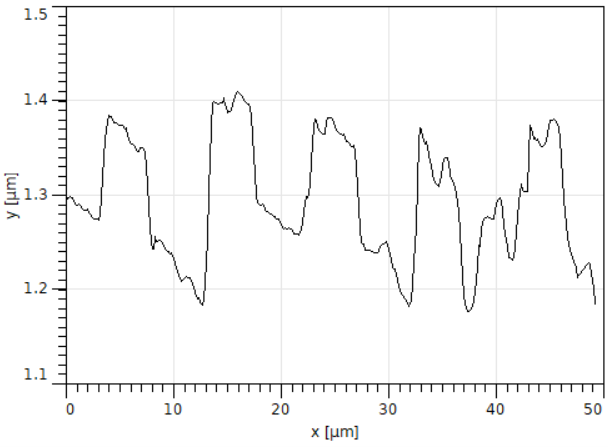
\includegraphics[scale = 0.65]{Bilder/zUngeeignet.png}
    \caption{Ungeeignetes Höhenprofil einer Geraden aus dem Ausschnitt des Eichgitters}
    \label{bild:zUngeeignet}
\end{figure}

\newpage
%Matteo Kumar - Leonhard Schatt
% Fortgeschrittenes Physikalisches Praktikum

% Teilauswertung CD

\section{Untersuchung eines CD-Presswerkzeugs}
\subsection{Bumphöhe}

Zunächst wird der 50$\mu m$-Ausschnitt zur Bestimmung der Bumphöhe untersucht.
Auf Abb. \ref{bild:CD50Linie} ist ein großer heller Fleck am unteren Bildrand zu erkennen. Dies könnte eine Verunreinigung wie z.B. Staub sein. 
Zur Bestimmung der Höhe der Bumps wird das Profil über mehrere Tracks betrachtet. 

\begin{figure}[h]
    \centering
    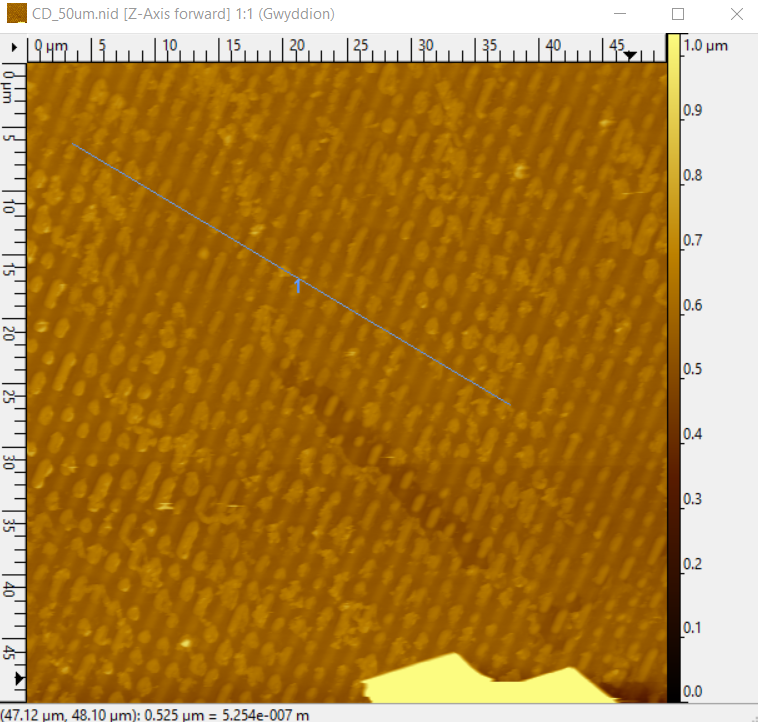
\includegraphics[scale = 0.47]{Bilder/CD50Linie.png}
    \caption{Aufnahme eines CD-Pressswerkzeugs auf 50x50 $\mu$m. Unten ist eine Verunreinigung als heller Fleck zu sehen. Die Strecke 
    für das benutzte Höhenprofil ist ebenfalls eingezeichnet}
    \label{bild:CD50Linie}
\end{figure}

\begin{figure}[h]
    \centering
    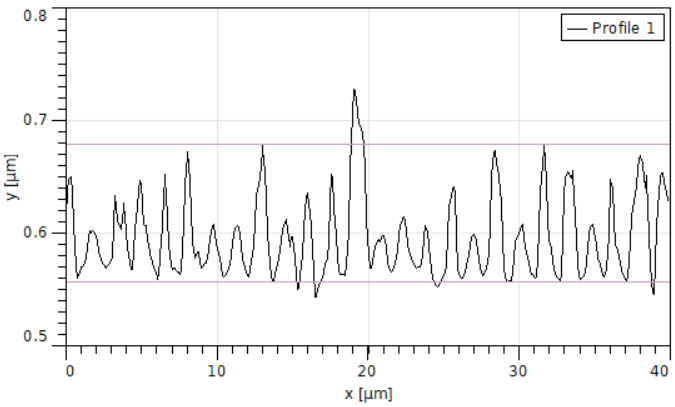
\includegraphics[scale = 0.6]{Bilder/CD50Profil.png}
    \caption{Höhenprofil durch die Bumps des CD-Presswerkzeuges. Als Anhaltspunkt für die Höhe der Bumps dienen die rosafarbenen Linien, die 
    122.2 nm auseinander sind.}
    \label{bild:CD50Profil}
\end{figure}

Die Höhe der Bumps soll mit Hilfe von Abb. \ref{bild:CD50Profil} eingeordnet werden. 
Die rosanen Linien stellen einen Abstand von 122.2 nm dar. Der große Bump hat eine Höhe von 164.4 nm. Der Hersteller 
gibt allerdings Höhen von ca. 200nm an (\cite{SampleKit2007}). Da die Ungenauigkeit des Herstellerwertes nicht bekannt ist, ist eine Einordnung an dieser Stelle 
schwierig. Allerdings ist durchaus zu erkennen, dass die gemessenen Bumps deutlich kleiner sind. Womöglich liegt auch hier bereits eine 
Abnutzung von einigen nm vor.
\newpage

\subsection{Trackabstand}

Nun wird der 20$\mu m$-Ausschnitt betrachtet. Es wird ein Höhenprofil entlang der in Abb. \ref{bild:CD20Linie} eingezeichneten Strecke 
erstellt. Zur Bestimmung des Trackabstandes wird das gesamte Profil über 12 Bumps hinweg gemessen, wie in Abb. \ref{bild:CD20Profil} zu 
sehen. 

\begin{figure}[h]
    \centering
    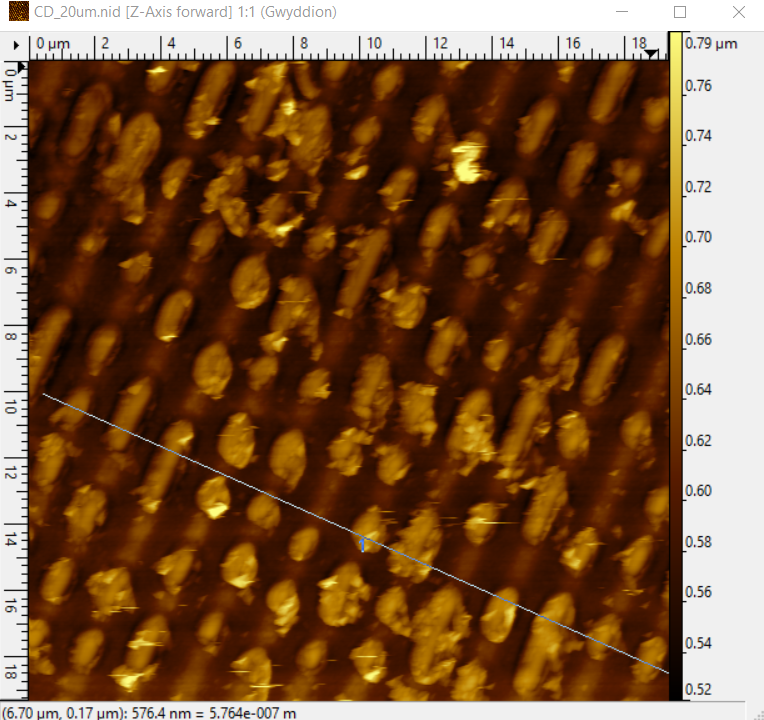
\includegraphics[scale = 0.5]{Bilder/CD20Linie.png}
    \caption{Aufnahme eines CD-Pressswerkzeugs auf 20x20 $\mu$m. Die Strecke 
    für das benutzte Höhenprofil ist ebenfalls eingezeichnet}
    \label{bild:CD20Linie}
\end{figure}

\begin{figure}[h]
    \centering
    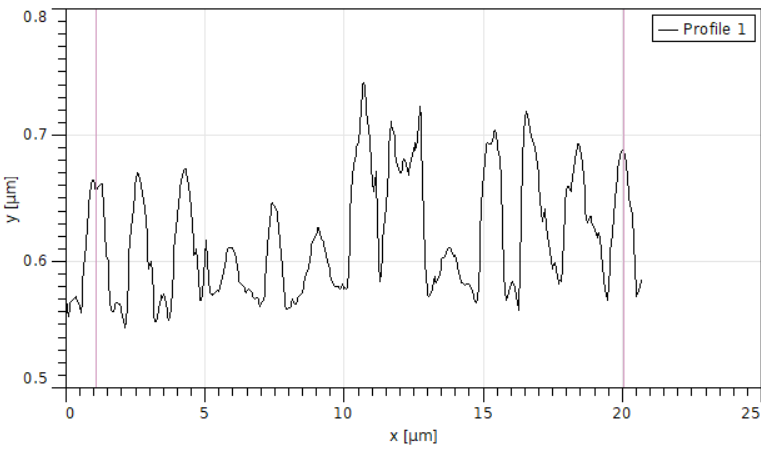
\includegraphics[scale = 0.6]{Bilder/CD20Profil.png}
    \caption{Profil durch die Bumps des Presswerkzeugs. Zur Ermittlung der Trackbreite wurde über 12 Bumps zwischen den rosafarbenen 
    Linien gemessen.}
    \label{bild:CD20Profil}
\end{figure}


Die rosanen Linien stellen einen Abstand von 18.981 $\mu$m dar. Das entspricht einem Trackabstand von $d_{Tr} = 1.582 \mu m$.
Der Fehler ergibt sich aus der Wahl der Veressungslinien, da die Mitte der Bumps nicht exakt bestimmt werden konnte, da die Spitzen und 
der Mittelpunkt zwischen Anstieg und Abfall der Bumps nicht immer übereinstimmen. Deshalb wird der Fehler für beide Linien anhand des 
Profils auf jeweils 0.3 $\mu$m geschätzt. Dies entspricht einem Fehler von 0.05 $\mu$m für den Mittelwert, wodurch sich für den Gesamtfehler ergibt: 
\begin{equation*}
    s = \sqrt{0.05^2 + (1.58 \cdot 0.012)^2}\, \mu m = 0.053\, \mu m
\end{equation*}

Damit ergibt sich der Trackabstand zu

\begin{equation*}
    \textcolor{red}{d_{Tr} = (1.58 \pm 0.06) \mu m}.
\end{equation*}

Der Hersteller gibt einen nominellen Wert von 1.6$\mu$m an (\cite{SampleKit2007}). 
Dieser liegt innerhalb des Fehlers; er wird also durch die Messung bestätigt.

\subsection{Bumplänge}

Als nächstes werden die Längen der Bumps ausgemessen. Dazu wird ein Höhenprofil entlang eines Tracks, wie in Abb. \ref{bild:CD20Laenge} 
gezeigt, angelegt.  

\begin{figure}[h]
    \centering
    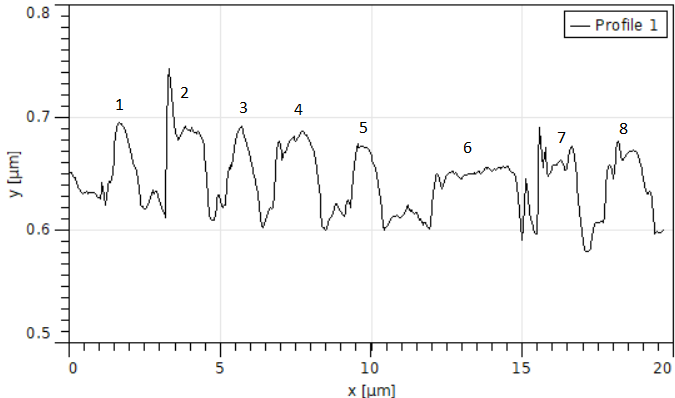
\includegraphics[scale = 0.8]{Bilder/CD20LaengeProfil.png}
    \caption{Profil durch die Bumps des Presswerkzeugs in Längsrichtung.}
    \label{bild:CD20LaengeProfil}
\end{figure}


\begin{figure}[h]
    \centering
    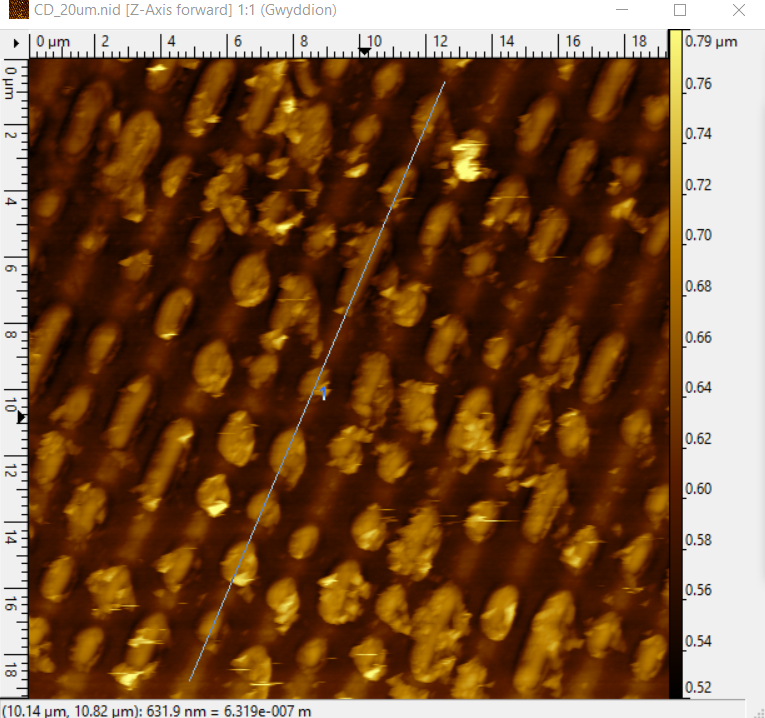
\includegraphics[scale = 0.5]{Bilder/CD20Laenge.png}
    \caption{Strecke entlang eines Tracks, entlang der das Profil zur Bestimmung der Länge der Bumps ermittelt wird.}
    \label{bild:CD20Laenge}
\end{figure}


\newpage

Auf diesem Profil (Abb. \ref{bild:CD20LaengeProfil}) sind acht größere Bumps erkennbar. Von links nach rechts 
sind deren Längen: 

\begin{center}
    \centering
    \begin{tabular}{l|r}
        Nummer Bump (v.l.n.r.) & Länge / $\mu$m \\
        \hline
        1 & 1.28 $\pm$ 1\\
        2 & 1.66 $\pm$ 1\\
        3 & 1.45 $\pm$ 1\\
        4 & 1.95 $\pm$ 1\\
        5 & 1.33 $\pm$ 1\\
        6 & 3.11 $\pm$ 1\\
        7 & 1.74 $\pm$ 1\\
        8 & 1.82 $\pm$ 1\\
        
    \end{tabular}
\end{center}

Die Längen der Bumps in dieser Auswahl liegen also alle im Bereich von 1.2-3.2$\mu$m. Laut Hersteller sollten die Längen in einer Spanne von 
0.8-3$\mu$m liegen (\cite{SampleKit2007}). 
Berücksichtigt man noch die Fehler beim Setzen der Markierungen beim Ausmessen der Bumps (abgeschätzt auf 1$\mu$m 
pro Markierung), so umfasst der angegebene Bereich noch die gemessenen Werte. 
\clearpage
%Matteo Kumar - Leonard Schatt
% Fortgeschrittenes Physikalisches Praktikum

% Teilauswertung Nanoröhrchen

\section{Nanoröhrchen}
Dieser Versuchsteil widmet sich der Untersuchung der Nanoröhrchen. Diese sind Kohlenstoffnanoröhre, welche auf einem Silizium-Waver 
fixiert wurden. Ziel diese Versuchsteiles ist es den Krümmungsradius der Spitze zu bestimmen.
\subsection{Länge und Durchmesser}
\subsubsection*{Länge}
Um die Länge einzelner Nanoröhrchen zu bestimmen, haben wir eine Aufnahme mit 15 $\mu$m als Seitenlängen gemacht. In dieser haben wir uns 
dann angeschaut, welche Längen unterschiedlich lange Kohlenstoffnanoröhren haben. Dazu bestimmt man mit dem Distanzmessen-Tool der Software 
"Gwyddion" die Länge möglichst gerader Nanoröhrchen bestimmt. \\
Die Abbildung \ref{Nanotube20} zeigt die oben genannte Aufnahme. Dabei kann man sehr schön die langgezogenen Fäden sehen. Welche dabei zum Vermessen verwendet wurden, 
kann man Abbildung \ref{Nanotube20Mess} im Anhang entnehmen.

\begin{figure}[h]
    \centering
    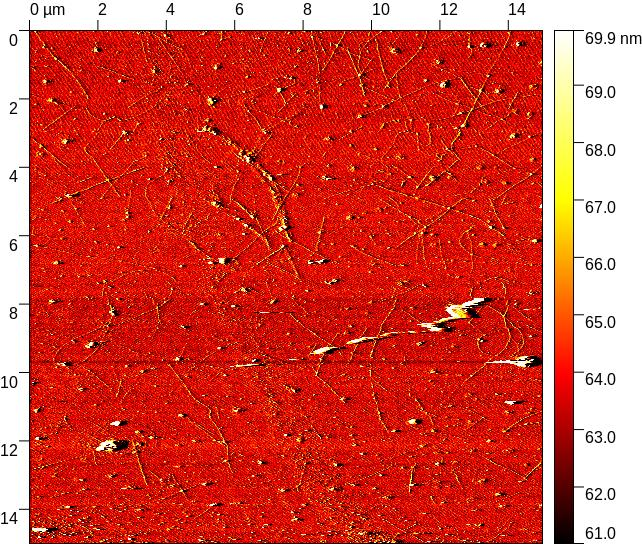
\includegraphics[width = 9cm]{Bilder/Nanotubes/NanoTube15um.jpg}
    \caption{Nanoröhrchen bei einer Bildgröße von 15x15$\mu$m}
    \label{Nanotube20}
\end{figure}

Dabei wurden folgende Werte aus Tabelle \ref{TabLaenge} gemessen. Die Fehlerrechnung kann man bei diesem 
Versuchsteil vernachlässigen, weil die Ablesefehler so groß sind, dass der Fehler des Messgeräts vernachlässigbar klein ist. Der Ablesefehler wird auf 15\% der Länge geschätzt. \\

\begin{table}
    \centering
    \begin{tabular}{lr}
        \toprule
        Röhrennummer &   Länge ($\mu$ m) \\
        \midrule
        0  &  2.883 $\pm$ 0.43 \\
        1  &  2.374 $\pm$ 0.35\\
        2  &  1.334 $\pm$ 0.20 \\
        3  &  3.050 $\pm$ 0.46 \\
        4  &  3.753 $\pm$ 0.56 \\
        5  &   0.860 $\pm$ 0.12\\
        6  &  1.583 $\pm$ 0.24 \\
        7  &  1.896 $\pm$ 0.28 \\
        8  &  1.542 $\pm$ 0.23 \\
        9  &   0.590 $\pm$ 0.075 \\
        10 &   0.464 $\pm$ 0.070 \\
        11 &  4.412 $\pm$ 0.66\\
        \bottomrule
    \end{tabular}
    \caption{Längenmessung der Nanoröhrchen. Der Ablesefehler wird auf 15\% der Länge geschätzt. \\
    }
    \label{TabLaenge}
\end{table}

Man erkennt, dass die Röhren sehr stark in ihrer Länge $l$  variieren.

\begin{equation}
    \textcolor{red}{\frac{l_{Min}}{l_{Max}} = 0.1053209772450975}
\end{equation}

Die maximale relative Unterschied in der Länge $l$ liegt bei einem Faktor 10. Dabei sind die Längen für die langen 
Nanoröhrchen, welche wir gemessen haben, noch nicht mal besonders lang. Diese können in Extremfällen bis zu
einen halben Meter lang werden (\cite{Dagani2002}).

\subsection*{Radius der Röhre}

Man muss sich Nanoröhrchen wie lange Röhren vorstellen, welche eine kreisförmige Grundfläche haben. Von dieser wollen wir nun den 
Radius bestimmen. Da das Abtasten aber einen Kreis mit anderem Radius ergibt muss man statt diesen Radius zu bestimmen, einfach 
den Höhenunterschied der des Hochpunktes der Röhre zum normalen untergrund bestimmen. Leider ist der Untergrund des Silizium-Wavers 
keineswegs glatt; deshalb ist es schwer den Unterschied exakt zu messen. Der Fehler im Ablesen der Werte dominiert den Fehler bei weitem. 
\begin{figure}
    \centering
    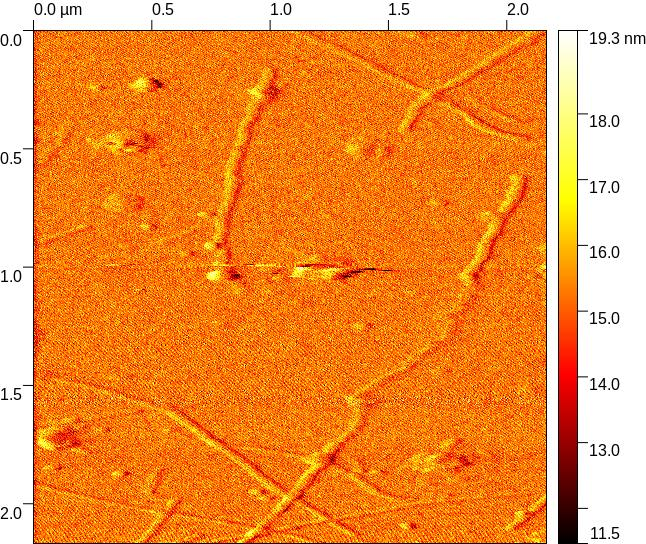
\includegraphics[width = 9cm]{Bilder/Nanotubes/NanoTube2um.jpg}
    \caption{Nanoröhrchen in einer Auflösung mit 512x512 Bildpunkten auf 2x2$\mu$m}
\end{figure}

Zur Bestimmung des Radius wird ein Röhrchen senkrecht mit einer Linie geschnitten. Auf dieser Linie betrachtet man dann das Höhenprofil der Aufnahme. Wir haben dafür die 
Linie, wie in Abbildung \ref{NanoRadius} zu sehen, gewählt. Damit erhält man den Querschnitt, der in Abbildung \ref{NanoQuerschnitt} 
dargestellt wird.

\begin{figure}
    \centering
    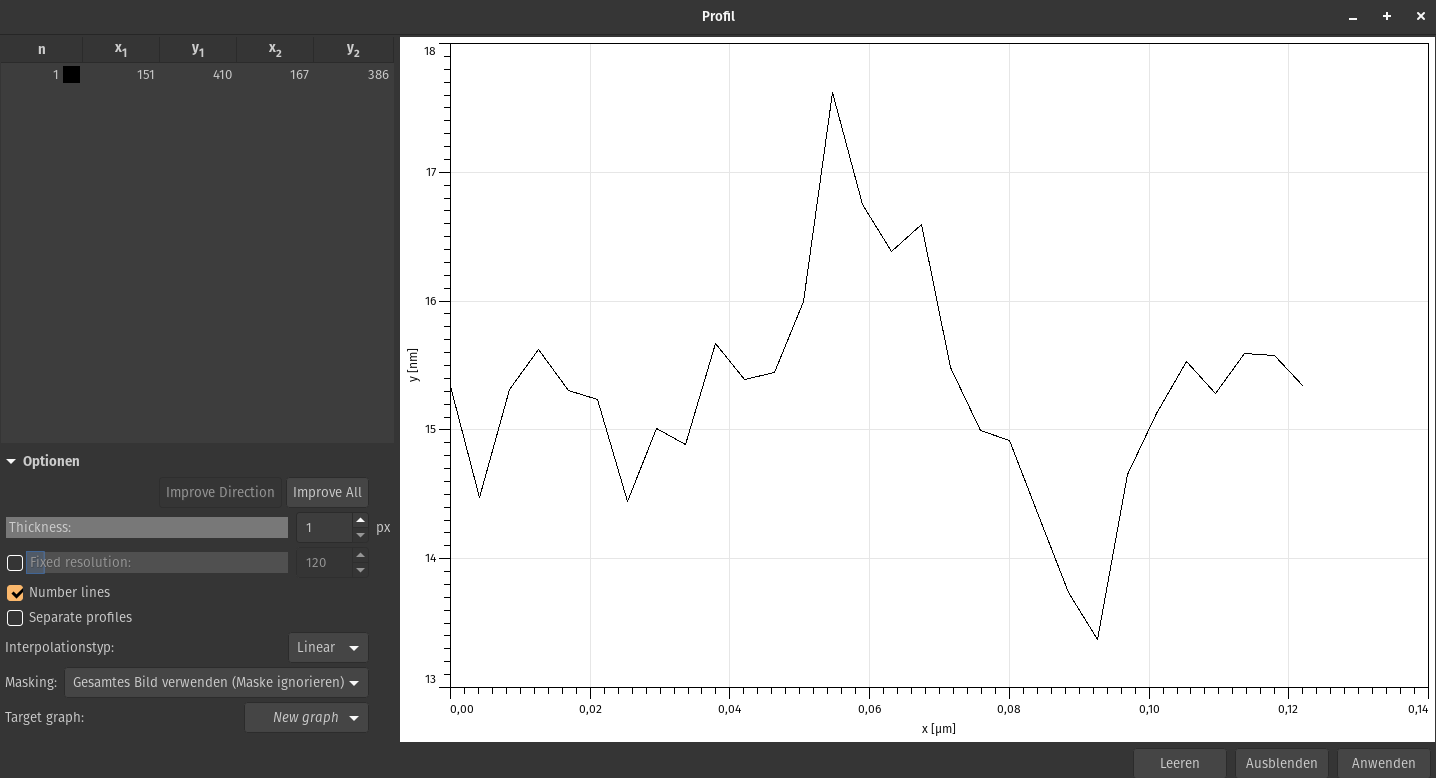
\includegraphics[width = \linewidth]{Bilder/Nanotubes/NanotubesBreiteHoehe.png}
    \caption{Querschnitt eins Kohlenstoffröhrchens}
    \label{NanoQuerschnitt}
\end{figure}

Aus diesem bestimmt man grafisch den Höhenunterschied. Dieser entspricht dann zwei Mal dem Radius $r$ der Röhre. Dabei wird der Fehler 
großzügig mit 15\% des Wertes angegeben.

\begin{equation*}
   r = \frac{\Delta z}{2} = \frac{2,6\mathrm{nm}}{2} = 1,3\mathrm{nm}
\end{equation*}

Durch das halbieren halbiert sich auch der Ablesefehler. 
\begin{equation*}
    \Rightarrow \textcolor{red}{r = (1,300 \pm 0,098)\mathrm{nm}}
\end{equation*}


\subsection{Krümmungsradius der Spitze des Cantilevers}

Wie oben beschrieben sagt die Form der Abtastung etwas über den Krümmungsradius der Spitze des Cantilevers aus. Das wird in Abbildung 
\ref{NanoTip} anschaulich dargestellt.

\begin{figure}
    \centering
    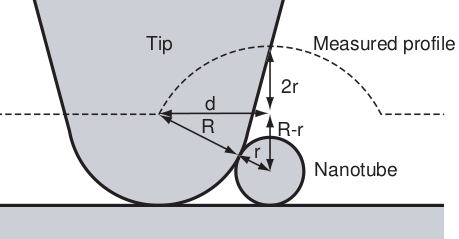
\includegraphics[width = 10cm]{Bilder/Nanotubes/TipGeoNano.png}
    \caption{Zusammenhang Krümmungsradius $R$ der Spitze und Präparatradius $r$ aus der abgebildeten Kontur (\cite[S.46]{SampleKit2007})}
    \label{NanoTip}
\end{figure}

Darau ergibt sich für den Radius der Spitze (\cite[S.47]{SampleKit2007}):\\
\begin{equation}
    R = \frac{d^2}{4r}
\end{equation}
mit $d$, $R$ und $r$ wie in Abbildung\ref{NanoTip} eingezeichnet.

Auch für $d$ setzt man beim Ablesen am besten ein großzügiges Intervall der Unsicherheit von 50\% an, da es schwer ist aus 
dem Rauschen herauszulesen, wo der Peak anfängt. Abgelesen wurde:\\

\begin{equation*}
    2d = 25,0\pm12,5\mathrm{nm} \Rightarrow d = (12,5\pm 6,3) \mathrm{nm} 
\end{equation*}

Daraus ergibt sich mit dem Fehlerfortpflanzungsgesetz:\\

\begin{equation}
    \textcolor{red}{R = (30\pm15) \mathrm{\,nm}}
\end{equation}

Das scheint ein in der Größenordnung realistischer Wert. Die Spitze könnte noch gut sein. Für eine Spitze sind Krümmungsradien zwischen 
10 und 20 nm normal. Die Spitze tendiert aber dazu, etwas abgenutzt zu sein.
\section{Gold}

Bei diesem Versuchsteil soll die Rauheit von Materialien genauer betrachtet werden. Diese gibt an, wie stark die Oberfläche von einer idealen, glatten Oberfläche abweicht. 
Dabei hätte eine ideal glatte Fläche eine Rauheit von 0nm. Je größer diese ist, desto rauer ist die Oberfläche.\\

Hier wird die Rauheit von Gold bestimmt. Dabei wird von einer Goldprobe die Rauheit in drei unterschiedlichen 
Aufnahmegrößen bestimmt. Diese werden dann verglichen und diskutiert.

Die entstehenden Bilder von Gold kann man im Anhang betrachten unter \ref{Gold1}, \ref{Gold2} und \ref{Gold3}.

Dabei erhält man für die Rauheit die folgenden Werte:\\
\begin{center}
    \centering
    \begin{tabular}{lr}
        \toprule
        Seitenlänge des Aufnahmebereichs ($\mu$m) & Rauheit (nm)\\
        \midrule
        2,5 & 1,335\\
        1,5 & 1,468 \\
        0,375 & 1,537\\
    \end{tabular}
\end{center}

Das Ergebnis ist zunächst kontraintuitiv. Man hätte erwartet, dass die Rauheit der Probe sinkt, 
wenn man näher heranzoomt. Aber gerade der gegenteilige Effekt ist zu beobachten. Dies ist damit zu erklären, 
dass bei größeren Ausschnitten das Abtasten nicht präzise genug ist, weil 
die Spitze zu schnell über die Probe lauft. Damit bekommt man kein vollständiges Bild der Probe, sondern nur einen groben Überblick. 
Um diese Hypothese zu überprüfen könnte man noch eine Referenzmessung machen. Bei dieser nimmt man dann den großen Ausschnitt und 
erhöht die Abtastzeit für eine Zeile massiv. Dann sollte man eine höhere Rauheit als die 
drei gemessenen Werte messen.
\clearpage
\section{PS/PMMA}

In diesem Teil der Auswertung wird demonstriert, warum die Information über die Phase beim AFM sehr aufschlussreich sein kann. Hier haben wir 
als Probe ein Gemisch aus Polystyrol und Polymethylmethacrylat. Diese wurden vermischt und dann auf einem Silizium-Waver aufgebracht. 
Jetzt fragt man sich im nachhinein, welches Material welches ist. Aus den topographischen Daten ist das leider nicht mehr ersichtlich. Abgesehen davon kann man auch 
nicht so gut unterscheiden, welcher Teil des Gemisches wo endet (siehe Abbildung \ref{PMMA1}).\\
\begin{figure}[h]
    \centering
    \includegraphics[width = 9cm]{Bilder/PMMA/PSPMMA.jpg}
    \caption{PS/PMMA in der Topographieansicht}
    \label{PMMA1}
\end{figure}

Betrachtet man nun aber das Phasenbild fällt auf, dass die Unterschied eindeutig zu sehen sind. Dabei gibt es sehr dunkle und helle Punkte 
in der Abbildung \ref{PMMA2}.\\

\begin{figure}
    \centering
    \includegraphics[width = 9cm]{Bilder/PMMA/PSPMMAPhase.jpg}
    \caption{Phaseninformation zur selben Aufnahmen wie in Abbildung \ref{PMMA1}}
    \label{PMMA2}
\end{figure}

Das liegt daran, dass beim Phasenkontrastmodus Informationen über die lokale Härte der Probe gesammelt werden. Man kann also 
Rückschlüsse auf die chemische Zusammensetzung beispielsweise machen, welche rein aus dem topographischen Daten nicht ersichtlich waren.\\
Dabei wird der Phasenkontrastmodus vor allem verwendet um einen guten Kontrast im Bild zu erzeugen und qualitative Aussagen zu machen. 
Für quantitative Aussagen ist er oft zu ungenau, da er von zu vielen oft nur ungefähr bekannten Größen wie Federkonstante, unterschiedlichen Kräften und Spitzengeometrie 
abhängt (\cite[S.68]{SampleKit2007}).
Hier kann man beispielweise sagen, dass die hellen Flecken Polystyrol sind, da dieses härter ist als Polymethylmethacrylat\footnotemark.
\footnotetext{\url{https://de.wikipedia.org/wiki/Polymethylmethacrylat}, Eingesehen am 22.09.2021}
%Matteo Kumar - Leonhard Schatt
% Fortgeschrittenes Physikalisches Praktikum

% Teilauswertung Oberflächengitter
\clearpage
\section{Gitterkonstante eines Oberflächengitters}

Als letzes wird noch ein Oberflächengitter vermessen, um dessen Gitterkonstante zu bestimmen. Dazu wird wieder ein Profil entlang der in 
Abb. \ref{bild:OFGitter} eingezeichneten Linie erstellt.

\begin{figure}[h]
    \centering
    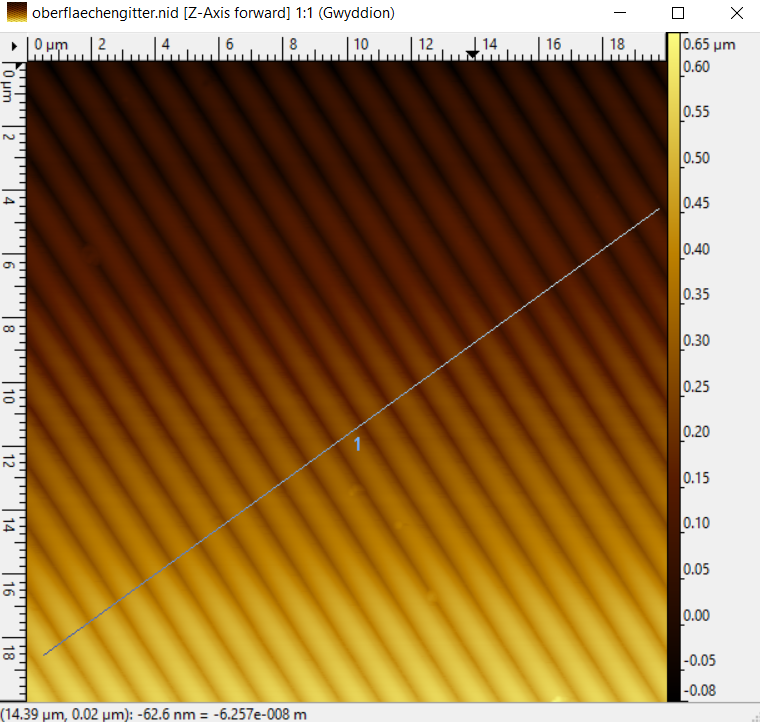
\includegraphics[scale = 0.45]{Bilder/OFGitter.png}
    \caption{Höhenprofil der ersten Geraden}
    \label{bild:OFGitter}
\end{figure}

\begin{figure}[ht]
    \centering
    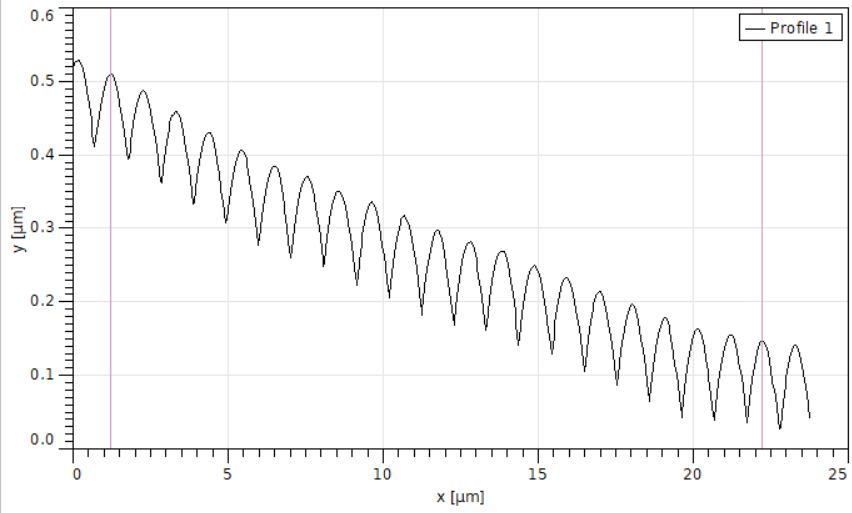
\includegraphics[scale = 0.55]{Bilder/OFGitterProfil.png}
    \caption{Höhenprofil der ersten Geraden}
    \label{bild:OFGitterProfil}
\end{figure}


Anschließend wird das Profil über 20 Kanten hinweg vermessen, wie in Abb. \ref{bild:OFGitterProfil} gezeigt. Die Gesamtlänge beträgt 
21.016 $\mu$m; der Mittelwert beträgt also 1.0508$\mu$m. 
Der Fehler liegt wieder in dem Setzen der Linien, zwischen denen gemessen wurde. Anhand des Abmess-Tools wird dieser auf 0.1$\mu$m pro 
Linie geschätzt. Für den Mittelwert ergibt sich demnach ein Fehler von 0.01$\mu$m. Der Gesamtfehler ergibt sich mit dem internen Fehler also zu
\begin{equation*}
    s = \sqrt{0.01^2 + (0.012 \cdot 1.0508)^2}\, \mu m = 0.016 \mu m
\end{equation*}
Die Gitterkonstante des Oberflächengitters beträgt also:
\begin{equation*}
    \textcolor{red}{g = (1.051 \pm 0.016) \mu m}
\end{equation*}



% etc.

    % 5.Kapitel Fazit
    %Matteo Kumar - Leonard Schatt
% Fortgeschrittenes Physikalisches Praktikum

% 5. Kapitel Einleitung

\chapter{Fazit}
\label{chap:fazit}
Wie in der Einleitung schon beschrieben ist FRET ein wichtiger Effekt, der vor allem in organischen Systemen auftritt. Dieser 
wurde uns in diesem Versuch näher gebracht. Das Auswerten ganzer Bilddateien mit 'Fiji' war auch eine neue Erfahrung, 
welche sicher in späteren Arbeiten noch eine Anwendung finden wird. Des Weiteren haben wir einen guten Einblick zu Fluorophoren bekommen; uns ist nun klar, dass
die Darstellung von leuchtenden Mäusen in biochemischen Laboren eine lächerliche Erfindung der Filmindustrie ist, da die Lebensdauer der angeregten 
Zustände sich im Nanosekundenbereich befindet. 



    % Anhang
    %% Matteo Kumar - Leonard Schatt
% Physikalisches Praktikum

% Anhang

\appendix

% Text

% Matteo Kumar - Leonard Schatt
% Physikalisches Praktikum

% Anhang A

\chapter{Anhang}
\label{chap:anhangA}
\section{FLIM}

\begin{figure}[h]
    \centering
    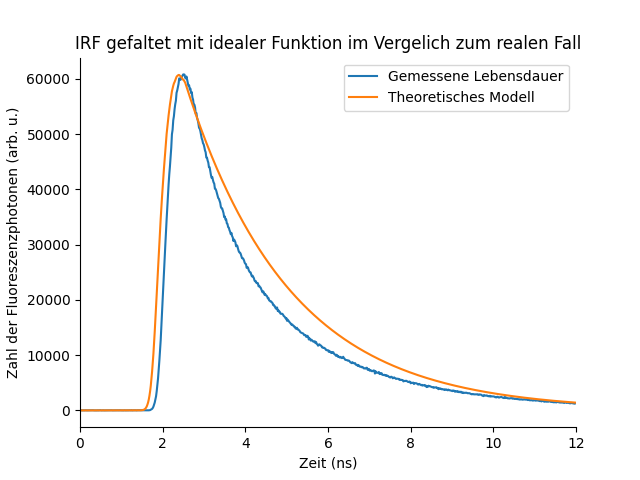
\includegraphics[width = \linewidth]{Bilder/Auswertung/IRFProgConvol.png}
    \caption{Lebensdauer bei Einzelphotonenereignissen und die Faltung der IRF (Programmgeneriert) und dem idealen Signal ($\tau_{YFP}$ unkorrigiert) nach der Totzeit. }
    \label{bild:IRFconvProg}
\end{figure}


\begin{figure}[h]
    \centering
    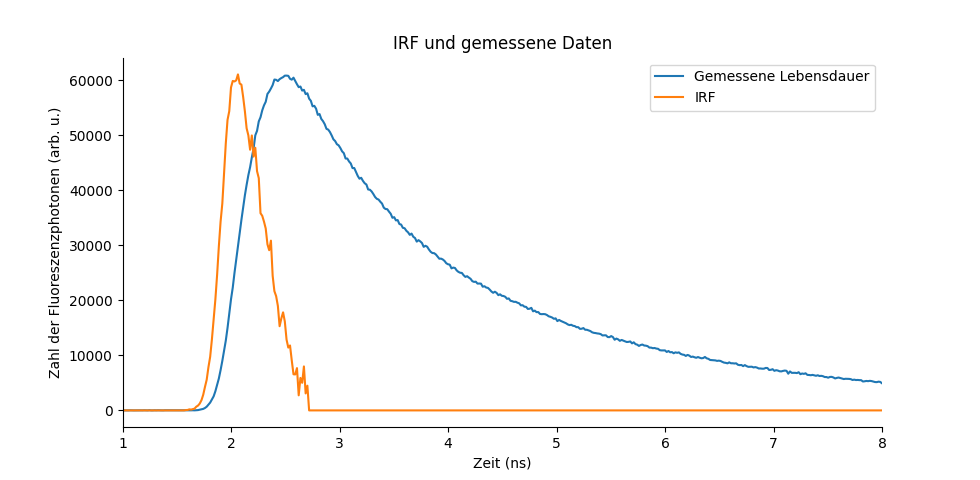
\includegraphics[width = \linewidth]{Bilder/Auswertung/IRFProg.png}
    \caption{ Lebensdauer bei Einzelphotonenereignissen und IRF durch das Programm 'SymPhoTime' generiert. Man sieht eine unsymmetrische Form.}
    \label{bild:IRFProg}
\end{figure}



\clearpage
\section{Protokoll}
\label{section:Protokoll}
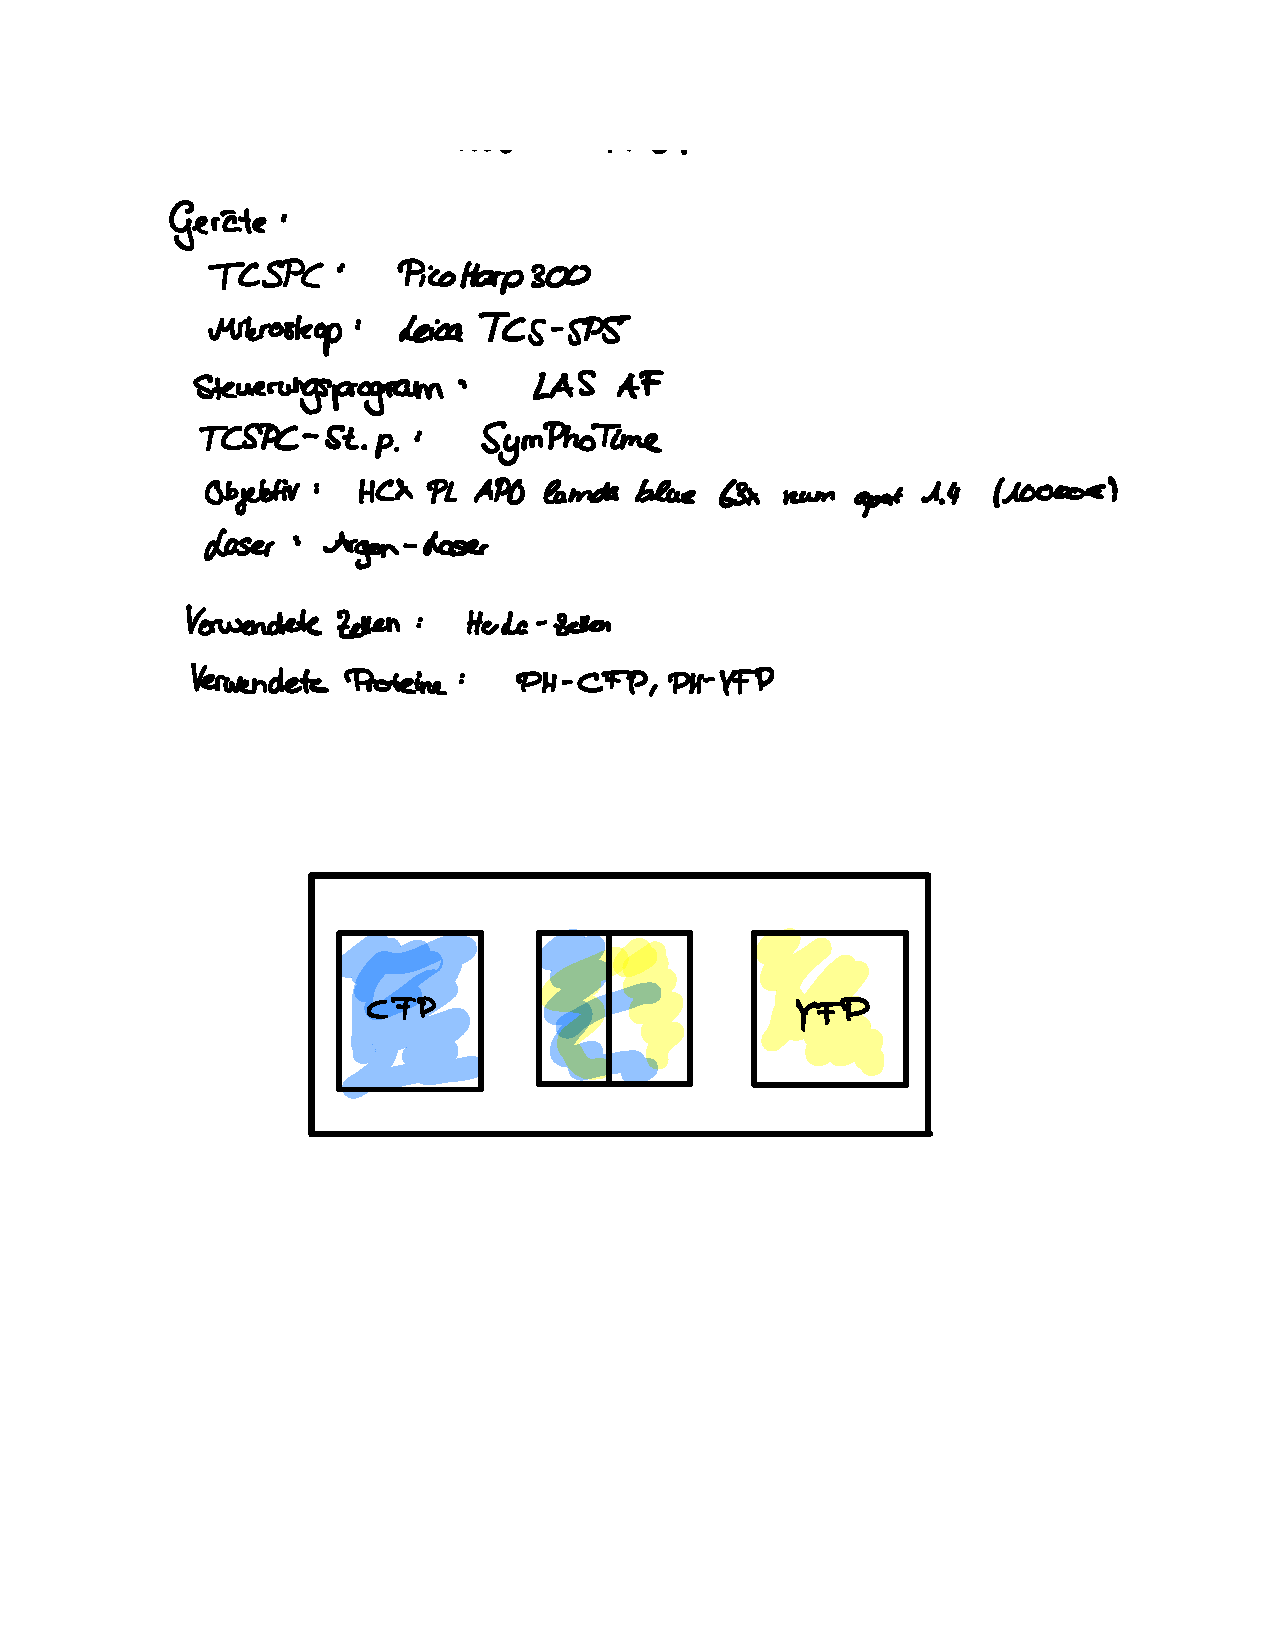
\includepdf[pages = 1-6]{FRETProt.pdf}



    % Literatur

    \bibliographystyle{Auswertung.bst}
    \bibliography{Auswertung.bib}

    %Abbildungsverzeichnis
    \listoffigures

\end{document}